% Basado en el template realizado por Diego Essaya, disponible en
%                                                         http://lug.fi.uba.ar
% Modificado por Sebastián Santisi.
% 2007: Modificado por Patricio Moreno y Michel Peterson.
% 2014: Modificado por Patricio Moreno.
% 2017: Modificado por Patricio Moreno.
% 2021: Modificado por Carla Sobico.
% 2024: Modificado(simplificado) por Francisco Del Rio.

% Acá se define el tamaño de letra principal:
% Para utilizar los estilos de KOMA-script, desconectar la línea siguiente y
% comentar la que le sigue (dejar sin comentar un único documentclass)
%\documentclass[10pt, spanish]{scrartcl}
\documentclass[a4paper, twoside, 10pt, spanish]{article}

%%%%%%%%%%%%%%%%%%%%%%%%%%%%%%
% CS
%%%%%%%%%%%%%%%%%%%%%%%%%%%%%%
\usepackage{listings}
\usepackage[version=4]{mhchem}
\usepackage{booktabs}
\usepackage[margin=1in]{geometry}
\usepackage{array}
\usepackage{pdflscape}
\usepackage{algorithm}
\usepackage{algpseudocode}
% CONFIGURACIONES GENERALES
%%%%%%%%%%%%%%%%%%%%%%%%%%%%%%%%%%%%%%%%%%%%%%%%%%%%%%%%%%%%%%%%%%%%%%%%%%%%%
% Definición del tamaño de página y los márgenes:
% Si preferís menos márgenes, descomentá la línea siguiente
%\usepackage[a4paper,headheight=16pt,scale={0.7,0.8},hoffset=0.5cm]{geometry}
\usepackage[demo]{graphicx}
\usepackage{caption}
\usepackage{subcaption}
\usepackage{babel}  % contiene la correcta separación en sílabas del español


\addto\captionsspanish{
  \renewcommand{\tablename}{Tabla}
} %Este comando hace que se use la palabra "Tabla" en lugar de "Cuadro" en las captions de las tablas.

\usepackage[utf8x]{inputenc}    % porque el encoding del documento es UTF-8
\usepackage[per-mode=fraction]{siunitx}
\sisetup%
{
	output-decimal-marker = {,},
	exponent-product = \cdot,
    group-digits = integer,
	group-separator = {.},
    locale = DE,
    round-mode = figures,
    round-precision = 3,
}


%
% El paquete amsmath agrega algunas funcionalidades extra a las fórmulas.
% Además defino la numeración de las tablas y figuras al estilo "Figura 2.3",
% en lugar de "Figura 7". (Por lo tanto, aunque no uses fórmulas, si querés
% este tipo de numeración dejá el paquete amsmath descomentado).
%
\usepackage{mathrsfs}
\usepackage{amsmath, amsfonts, amssymb}
%\numberwithin{equation}{section}
%\numberwithin{figure}{section}
\numberwithin{table}{section}
%%%%%%%%%%%%%%%%%%%%%%%%%%%%%%%%%%%%%%%%%%%%%%%%%%%%%%%%%%%%%%%%%%%%%%%%%%%%%

%%%%%%%%%%%%%%%%%%%%%%%%%%%%%%%%%%%%%%%%%%%%%%%%%%%%%%%%%%%%%%%%%%%%%%%%%%%%%
% ENCABEZADO y PIE DE PÁGINA
%%%%%%%%%%%%%%%%%%%%%%%%%%%%%%%%%%%%%%%%%%%%%%%%%%%%%%%%%%%%%%%%%%%%%%%%%%%%%
\usepackage{fancyhdr}   % Para poder personalizarlo
\usepackage{lastpage}   % Para poder saber cuántas páginas tiene el documento
\pagestyle{fancy}
\renewcommand{\sectionmark}[1]{\markboth{}{\thesection\ \ #1}}
\fancyhead{}	% Elimino el contenido del encabezado
% Muestra la sección a la derecha (izquierda) en páginas impares (pares)
\fancyhead[RO,LE]{\rightmark}
% El siguiente texto a la derecha (izquierda) en páginas pares (impares)
\fancyhead[RE,LO]{TB070 - Trabajo Práctico Final}
\fancyfoot{}	% Elimino el contenido del pie de página
% A la izquierda (derecha) en páginas pares (impares): nro. de página / total
\fancyfoot[LE,RO]{\thepage/\pageref{LastPage}}
%%%%%%%%%%%%%%%%%%%%%%%%%%%%%%%%%%%%%%%%%%%%%%%%%%%%%%%%%%%%%%%%%%%%%%%%%%%%%

%%%%%%%%%%%%%%%%%%%%%%%%%%%%%%%%%%%%%%%%%%%%%%%%%%%%%%%%%%%%%%%%%%%%%%%%%%%%%
% Hipervínculos (enlaces) en el documento (y modificación de atributos)
%%%%%%%%%%%%%%%%%%%%%%%%%%%%%%%%%%%%%%%%%%%%%%%%%%%%%%%%%%%%%%%%%%%%%%%%%%%%%
\usepackage{url}
\urlstyle{tt}
\usepackage[colorlinks=true,linkcolor=black, urlcolor=blue]{hyperref}
\hypersetup{
    breaklinks,
    baseurl       = http://,
    pdfborder     = 0 0 0,
    pdfpagemode   = UseNone,
    pdfstartpage  = 1,
    pdfcreator    = {Plantilla de informe de TP para \LaTeX{}},
    bookmarksopen = true,
    bookmarksdepth= 2,% to show sections and subsections
    pdfauthor     = {Apellido~1, Apellido~2, Apellido~3},
    pdftitle      = {-},
    pdfsubject    = {Informe},
    pdfkeywords   = {}%
    }

%%%%%%%%%%%%%%%%%%%%%%%%%%%%%%%%%%%%%%%%%%%%%%%%%%%%%%%%%%%%%%%%%%%%%%%%%%%%%

%%%%%%%%%%%%%%%%%%%%%%%%%%%%%%%%%%%%%%%%%%%%%%%%%%%%%%%%%%%%%%%%%%%%%%%%%%%%%
% LISTAS (para poder modificar los 'bullets' de las listas)
%%%%%%%%%%%%%%%%%%%%%%%%%%%%%%%%%%%%%%%%%%%%%%%%%%%%%%%%%%%%%%%%%%%%%%%%%%%%%
\usepackage{enumerate}
%%%%%%%%%%%%%%%%%%%%%%%%%%%%%%%%%%%%%%%%%%%%%%%%%%%%%%%%%%%%%%%%%%%%%%%%%%%%%

%%%%%%%%%%%%%%%%%%%%%%%%%%%%%%%%%%%%%%%%%%%%%%%%%%%%%%%%%%%%%%%%%%%%%%%%%%%%%
% TABLAS (para que se vean bien)
%%%%%%%%%%%%%%%%%%%%%%%%%%%%%%%%%%%%%%%%%%%%%%%%%%%%%%%%%%%%%%%%%%%%%%%%%%%%%
\usepackage{booktabs}
\usepackage{multirow}
%%%%%%%%%%%%%%%%%%%%%%%%%%%%%%%%%%%%%%%%%%%%%%%%%%%%%%%%%%%%%%%%%%%%%%%%%%%%%

%%%%%%%%%%%%%%%%%%%%%%%%%%%%%%%%%%%%%%%%%%%%%%%%%%%%%%%%%%%%%%%%%%%%%%%%%%%%%
% IMÁGENES
%%%%%%%%%%%%%%%%%%%%%%%%%%%%%%%%%%%%%%%%%%%%%%%%%%%%%%%%%%%%%%%%%%%%%%%%%%%%%
% Para incluir imágenes, el siguiente código carga el paquete graphicx
% según se esté generando un archivo dvi o un pdf (con pdflatex).

% Para generar dvi, descomentá la linea siguiente:
%\usepackage[dvips]{graphicx}

% Para generar pdf, descomentá las dos lineas seguientes:
\usepackage{graphicx}
\pdfcompresslevel=9

% Todas las imágenes están en el directorio imgs:
\newcommand{\imgdir}{imgs}
\graphicspath{{\imgdir/}}
%%%%%%%%%%%%%%%%%%%%%%%%%%%%%%%%%%%%%%%%%%%%%%%%%%%%%%%%%%%%%%%%%%%%%%%%%%%%%

%%%%%%%%%%%%%%%%%%%%%%%%%%%%%%%%%%%%%%%%%%%%%%%%%%%%%%%%%%%%%%%%%%%%%%%%%%%%%
% DIAGRAMAS DE FLUJO EN DIA
%%%%%%%%%%%%%%%%%%%%%%%%%%%%%%%%%%%%%%%%%%%%%%%%%%%%%%%%%%%%%%%%%%%%%%%%%%%%%
% Necesitas este paquete si haces los diagramas de flujo en el programa Dia
% y exportás a latex
%\usepackage{tikz}
%%%%%%%%%%%%%%%%%%%%%%%%%%%%%%%%%%%%%%%%%%%%%%%%%%%%%%%%%%%%%%%%%%%%%%%%%%%%%

%%%%%%%%%%%%%%%%%%%%%%%%%%%%%%%%%%%%%%%%%%%%%%%%%%%%%%%%%%%%%%%%%%%%%%%%%%%%%
% INSERCIÓN DE CÓDIGO FUENTE
%%%%%%%%%%%%%%%%%%%%%%%%%%%%%%%%%%%%%%%%%%%%%%%%%%%%%%%%%%%%%%%%%%%%%%%%%%%%%
% El código aparece solo en blanco y negro, lo que es más comodo para la impresión
%%%%%%%%%%%%%%%%%%%%%%%%%%%%%%%%%%%%%%%%%%%%%%%%%%%%%%%%%%%%%%%%%%%%%%%%%%%%%
% COMANDOS UTILES
%%%%%%%%%%%%%%%%%%%%%%%%%%%%%%%%%%%%%%%%%%%%%%%%%%%%%%%%%%%%%%%%%%%%%%%%%%%%%
% los siguientes comandos permiten escribir de manera uniforme en todo el
% documento

% Para poder manejar los espacios al final de los comandos propios
\usepackage{xspace}

% Abreviatura de 'número' utilizando letras voladas (correcto español)
\newcommand{\Nro}{N.\textsuperscript{o}\xspace}
\newcommand{\nro}{n.\textsuperscript{o}\xspace}
%%%%%%%%%%%%%%%%%%%%%%%%%%%%%%%%%%%%%%%%%%%%%%%%%%%%%%%%%%%%%%%%%%%%%%%%%%%%%
% PAQUETES EXTRAS
%%%%%%%%%%%%%%%%%%%%%%%%%%%%%%%%%%%%%%%%%%%%%%%%%%%%%%%%%%%%%%%%%%%%%%%%%%%%%
\usepackage{circuitikz}
\usepackage{float}
\usepackage{multicol}
%\usepackage{pdfpages}
%\usepackage{subfigure}
%\usepackage{graphicx}%
\usepackage{gensymb}

\raggedbottom
%%%%%%%%%%%%%%%%%%%%%%%%%%%%%%%%%%%%%%%%%%%%%%%%%%%%%%%%%%%%%%%%%%%%%%%%%%%%%
%%%%%%%%%%%%%%%%%%%%%%%%%%%%%%%%%%%%%%%%%%%%%%%%%%%%%%%%%%%%%%%%%%%%%%%%%%%%%
% INICIO DEL DOCUMENTO
%%%%%%%%%%%%%%%%%%%%%%%%%%%%%%%%%%%%%%%%%%%%%%%%%%%%%%%%%%%%%%%%%%%%%%%%%%%%%
%%%%%%%%%%%%%%%%%%%%%%%%%%%%%%%%%%%%%%%%%%%%%%%%%%%%%%%%%%%%%%%%%%%%%%%%%%%%%
\begin{document}

% Hago que las páginas se comiencen a contar a partir de aquí:
%
\setcounter{page}{1}

%
% Carátula:
%
%\begin{titlepage}

\begin{center} % Modificar el código de ser necesario
{\underline{\textsc{Dispositivos Semiconductores [TB070]}}}\\
 {\textsc{Trabajo Práctico Final}}
\end{center}

 \begin{tabbing}
% %	FECHA : DD/MM/2019\\% \today\\
%TUTOR: Lorem ipsum dolor sit amet, \\
 \\
	ESTUDIANTE:\hspace{-1cm}\=\+\hspace{1cm}\=\hspace{6cm}\=\\	\>\>
              \\
              Del Rio, Francisco	\>\> 110761\\ 
              \>\footnotesize{\verb!fadelrio@fi.uba.ar!}\\
           
 \end{tabbing}


\hrule
\vspace{0.2cm}

% Modificar código de ser necesario
%\noindent\small{86.09 - Procesos Estocásticos \hfill}

%\tableofcontents
%\end{titlepage}

%

%

%
% Fin carátula
%

\DeclareSIUnit\angstrom{\text {Å}}

% Inicio del TP:
%%%%%%%%%%%%%%%%%%%%%%%%%%%%%%%%%%%%%%%%%%%%%%%%%%%%%%%%%%%%%%%%%%%%%%%%%%%%%%%%%%%%%%%%%%%%%%
\section{Resumen}

\quad Se inicia con parámetros constructivos de un MOSFET de canal largo, con los que se obtienen los parámetros de la estructura para luego poner a prueba los modelos numérico, cuadrático y clasico que permiten obtener la corriente que circula a traves del dispositivo. 

\quad Luego se reduce el tamaño del transistor usando una guia de escalado ''a campo eléctrico constante". Para este caso se estudian principalmente los efectos de canal corto, como modulacion de largo de canal, reduccion de barrera inducida por drain, degradación de la movilidad y saturacion de velocidad de arraste. Se obtiene un modelo final que tiene en cuenta todos los efectos de canal corto y permite una representación viable para el diseño con el transistor. 
%%%%%%%%%%%%%%%%%%%%%%%%%%%%%%%%%%%%%%%%%%%%%%%%%%%%%%%%%%%%%%%%%%%%%%%%%%%%%%%%%%%%%%%%%%%%%%
\section{Introducción}

\quad Un MOSFET o Metal-Oxide-Semiconductor Field-Effect Transistor es, como dice su nombre, un dispositivo semiconductor de la familia de los transistores basado en una juntura Metal-Oxido-Semiconductor. La caracteristica principal de un transistor es su capacidad de controlar el paso de corriente a traves de sus terminales, en el caso del MOSFET se controla la corriente que circula entre el Drain y el Source a traves de la diferencia de potencial aplicada entre el Gate y el Source. Resulta de interés modelar el comportamiento de este tipo de dispositivos, para su diseño y aplicacion en circuitos.

\quad Para esto ultimo existen distintos modelos, algunos más exhaustivos que otros, algunos con soluciones analíticas y otros que solo se pueden resolver con métodos numéricos. A su vez, las propiedades fisicas de construcción del dispositivo pueden dar lugar a fenómenos más complejos, que también son modelados y se pueden tener en cuenta a la hora de diseñar. 

\quad El objetivo de este trabajo es analizar las distintas formas de modelar un MOSFET, tanto de canal largo como de canal corto, con una gran parte de los efectos que se añaden en este último caso. 

%%%%%%%%%%%%%%%%%%%%%%%%%%%%%%%%%%%%%%%%%%%%%%%%%%%%%%%%%%%%%%%%%%%%%%%%%%%%%%%%%%%%%%%%%%%%%%

\section{Parte I: transistor canal largo}

\subsection{Parámetros de la estructura MOS}

Los datos fisicos del MOSFET provistos por la cátedra son: 

\begin{table}[ht] 
	\centering
	 \begin{tabular}{c c c c c c c c}
	 	 \hline \# &
	 	  $t_{ox}\,[\mathrm{nm}]$ &
	 	   $L\,[\mathrm{\mu m}]$ &
	 	    $W\,[\mathrm{\mu m}]$ &
	 	     $N_a\,[\mathrm{cm}^{-3}]$ &
	 	      $V_{DD}\,[\mathrm{V}]$ &
	 	       $r_j\,[\mathrm{nm}]$ &
	 	        $E_0 - E_{f_{\mathrm{poly}}}\,[\mathrm{eV}]$ \\ 
	 	        \hline 
	 	        \\
	 	        1 & 30 & 2{,}0 & 20 & $7 \times 10^{15}$ & 6{,}0 & 410 & 4{,}09 \\ \hline \end{tabular} \caption{Parámetros fisicos del dispositivo.} \label{tab:parametros-dispositivo} \end{table}

\paragraph{Cálculo de $\mu_{n_p}$}

Para la obtención de la movilidad se utilizó la siguiente formula 

\begin{equation*}
	\mu_{n_p}(N_a) = \mu_{min} + \frac{\mu_{max} - \mu_{min}}{1+\left(\frac{N_a}{N_{ref}}\right)^\alpha}
\end{equation*}

Donde los valores típicos del silicio son $\mu_{min} = \SI{68.5}{\per\cubic\centi\meter}$ , $\mu_{max} = \SI{1414}{\per\cubic\centi\meter}$ , $N_{ref} = \SI{9.2e16}{\per\cubic\centi\meter}$ y $\alpha = \SI{0.711}{}\\$

\paragraph{Cáclulo de $C_{ox}$:}

La capacidad del oxido se define de forma genérica como: 
\begin{equation*}
	C'_{ox} = \frac{\epsilon_{ox}}{t_{ox}}
\end{equation*}
Para luego relacionarse con las dimensiones del dipositivo y asi obtener el valor específico: 

\begin{equation*}
	C_{ox} = C'_{ox} W L.
\end{equation*}

El valor de $C'_{ox}$ obtenido es de \SI{115.05}{\nano\farad\per\centi\metre\squared}.

\paragraph{Cálculo de $\psi_B$:}

EL potencial viene dado por: 

\begin{equation*}
	\psi_B = -V_{TH} \log\left(\frac{N_a}{n_i}\right).
\end{equation*}

\paragraph{Cálculo de $\phi_{poly}$:}

Se trata de la diferencia de potencial entre el nivel de fermi del polisilicio y la energía de electron libre, por lo que se puede obtener de la siguiente forma: 

\begin{equation*}
	\phi_{poly} = \frac{E_0 - E_{f_{poly}}}{q}.
\end{equation*}

\paragraph{Cálculo de $\phi_s$:}

Es la diferencia de potencial entre el nivel de fermi del silicio y la energia de electron libre. Para el caso de silicio tipo p, donde la energia de fermi se encuentra entre el nivel intrinseco y la banda de valencia, se puede obtener como el potencial entre la banda de conduccion y la energia de electron libre más el potencial de el nivel intrinseco respecto a la banda de conduccion y el potencial del nivel de fermi respecto al nivel intrinseco:

\begin{equation*}
	\phi_s = \chi_{si} + \frac{E_g}{2 q} - \psi_B.
\end{equation*}

\paragraph{Cálculo de $\phi_{\mathrm{BI}(GB)}$:}

Para un metal, el potencial de built in viene definido por: 

\begin{equation*}
	\phi_{\mathrm{BI}(metal)} = \chi + \frac{E_g}{2q} + V_{TH} \log\left(\frac{N_a}{n_i}\right) - \phi_m.
\end{equation*}

Al tratarse de un gate de polisilicio $n^{+}p$, la energia del nivel de fermi es igual a la de la banda de conducción, el potencial $\phi_m = \chi$, por lo que se obtiene:

\begin{equation*}
		\phi_{\mathrm{BI}(GB)} =\frac{E_g}{2q} + V_{TH} \log\left(\frac{N_a}{n_i}\right).
\end{equation*} 

\paragraph{Cálculo de $V_{FB}$:}

La tensión de flatband es la tensión que, aplicada al gate, elimina la curvatura de las bandas. Viene definida por: 

\begin{equation*}
	V_{FB} = - \phi_{\mathrm{BI}(GB)}.
\end{equation*}

\paragraph{Cálculo de $\gamma$:}

Es un parámetro que indica el impacto de las tensiones aplicadas en el gate en el espesor del canal formado, viene dado por: 

\begin{equation*}
	\gamma = \frac{\sqrt{2 q N_a \epsilon_s}}{C'_{ox}}.
\end{equation*}

\paragraph{Cálculo de $V_T$:} 

La tensión umbral viene dada por: 

\begin{equation*}
	V_T = V_{FB} - 2 \psi_B + \gamma \sqrt{-2 \psi_B}.
\end{equation*}

\paragraph{Cálculo de m:}

Viene dado por: 

\begin{equation*}
	1 + \frac{\gamma}{2 \sqrt{-2 \psi_B}}.
\end{equation*}

La inversa de esta magnitud es una medida de la eficiencia de $V_{GS}$ para modular a $\psi_s$, por lo tanto, se busca que su valor sea lo mas cercano a 1 posible.

\paragraph{Resultados:}

En la siguiente tabla se presentan los valores obtenidos para cada una de las magnitudes previamente mencionadas.

\begin{table}[H]
	\centering
	\renewcommand{\arraystretch}{1.3}
	\caption{Parámetros obtenidos.}
	\begin{tabular}{lc}
		\toprule
		\textbf{Parámetro} & \textbf{Valor} \\
		\midrule
		$\mu_{np}$ & \SI{1228.35}{\centi\meter\squared\per\volt\per\second} \\
		$C_{ox}$ & \SI{46.02}{\femto\farad} \\
		$\psi_B$ & \SI{-0.3482}{\volt} \\
		$\phi_{\mathrm{poly}}$ & \SI{4.09}{\volt} \\
		$\phi_s$ & \SI{4.9182}{\volt} \\
		$\phi_{\mathrm{BI}(GB)}$ & \SI{0.9082}{\volt} \\
		$V_{FB}$ & \SI{-0.9082}{\volt} \\
		$\gamma$ & $0.4189\,\sqrt{\si{\volt}}$ \\
		$V_T$ & \SI{0.1378}{\volt} \\
		$m$ & \num{1.2510} \\
		\bottomrule
	\end{tabular}
\end{table}

\subsection{Curva $\psi_{s,d}$ vs $V_{DS}$}

\quad Patiendo desde la ecuacion del campo dentro del dispositivo: 

\begin{equation}\label{eq_campo_cuad}
	\mathscr{E}_s^2 = \frac{2q V_{th} N_a}{\epsilon_{si}} \left[ \left( exp(-\frac{\psi_{sd}}{V_{th}}) + \frac{\psi_{sd}}{V_{th}} -1 \right) + \frac{n_i^2}{N_a ^2}\left( exp\left( \frac{-V_{ds}}{V_{th}} \right) \left( exp \left( \frac{\psi_{sd}}{V_{th}}\right) -1\right) - \frac{\psi_{sd}}{V_{th}} \right) \right]
\end{equation}

Planteando la carga:

\begin{equation}\label{eq_carga}
	C_{ox}(V_{gs}-V_{FB} - \psi_{sd}) + Q'_s = 0
\end{equation}

y recordando la ley de Gauss:

\begin{equation}\label{eq_gauss}
	\mathscr{E}_s^2 = \left(\frac{Q'_s}{\epsilon_{si}}\right)^ 2
\end{equation}

Se puede definir a (\ref{eq_campo_cuad}) como $F(\psi_{s,d}, V_{DS})$ y utilizando (\ref{eq_gauss}) reemplazarlo en (\ref{eq_carga}). De esta forma, dado un $V_{DS}$ se puede ajustar un $\psi_{s,d}$ que sea la raiz de la ecuación. 

A continuación, el gráfico obtenido al obtener los $\psi_{s,d}$ para cuatro valores de $V_{GS}$ y para $V_{DS}$ entre \SI{0}{} y $V_{DD}$. Además, se superpone la curva $V_{DS} - 2 \psi_B$


\begin{figure}[H]
    \centering
    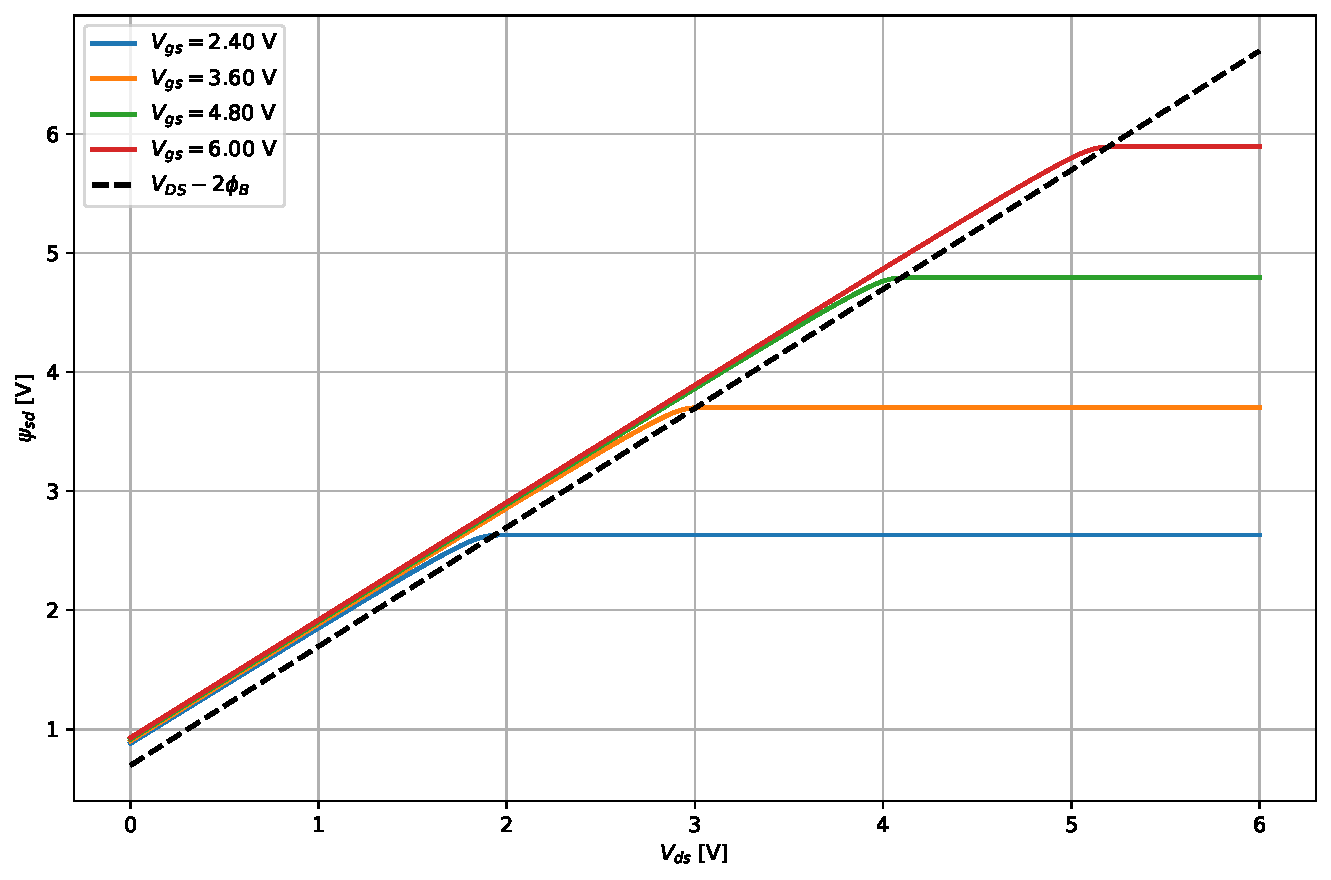
\includegraphics[width=0.7\linewidth]{res/phisd_vs_vds.pdf}
    \caption{Curvas de $\psi_{s,d}$ contra $V_{DS}$}
    \label{fig:phisd_vs_vds}
\end{figure}

\subsection{Cálculo de la curva de salida $I_D$ vs. $V_{DS}$}

La curva de salida permite ver el comportamiento del transistor para una tension de compuerta fija si varía la tensión aplicada entre las terminales Drain y Source. 

\subsubsection{Método numérico}

La corriente que circula por el terminal drain viene dada por la siguiente ecuación: 

\begin{equation}\label{eq:Id_gral}
	I_D = \mu_n \frac{W}{L}\{C'_{ox}(V_{GS}-V_{FB} + V_{TH})\psi_s-\frac{1}{2}C'_{ox} \psi_s ^2 -\frac{2}{3}\sqrt{2\epsilon_s q N_a}\psi_s^{\frac{3}{2}} + V_{th}\sqrt{2 \epsilon_s q N_a\psi_s}\}\left.\right|^{\psi_s = \psi_{sd}}_{\psi_s = \psi_{ss}}.
\end{equation}

Esta ecuación se evalúa en los puntos obtenidos en la subsección anterior, $\psi_{sd}$ es el valor para el par $V_{GS},V_{DS}$ correspondiente, y $psi_{ss}$ es el valor que corresponde al $V_{GS}$ de interés, pero con $V_{DS} = \SI{0}{\volt}$

La curva que separa el régimen de operacion lineal del de saturacion se conoce como curva de saturación, y está formada por los pares $I_{D(sat)}$ y $V_{DS(sat)}$. Los valores de $V_{DS(sat)}$ se pueden obtener buscando las intersecciones de las curvas de $\psi_{s,d}$ con la curva de $V_{DS} - 2 \psi_B$ de la \autoref{fig:phisd_vs_vds}.

A continuación el gráfico obtenido para los cuatro valores de $V_{GS}$ con la curva de saturacion superpuesta:

\begin{figure}[H]
    \centering
    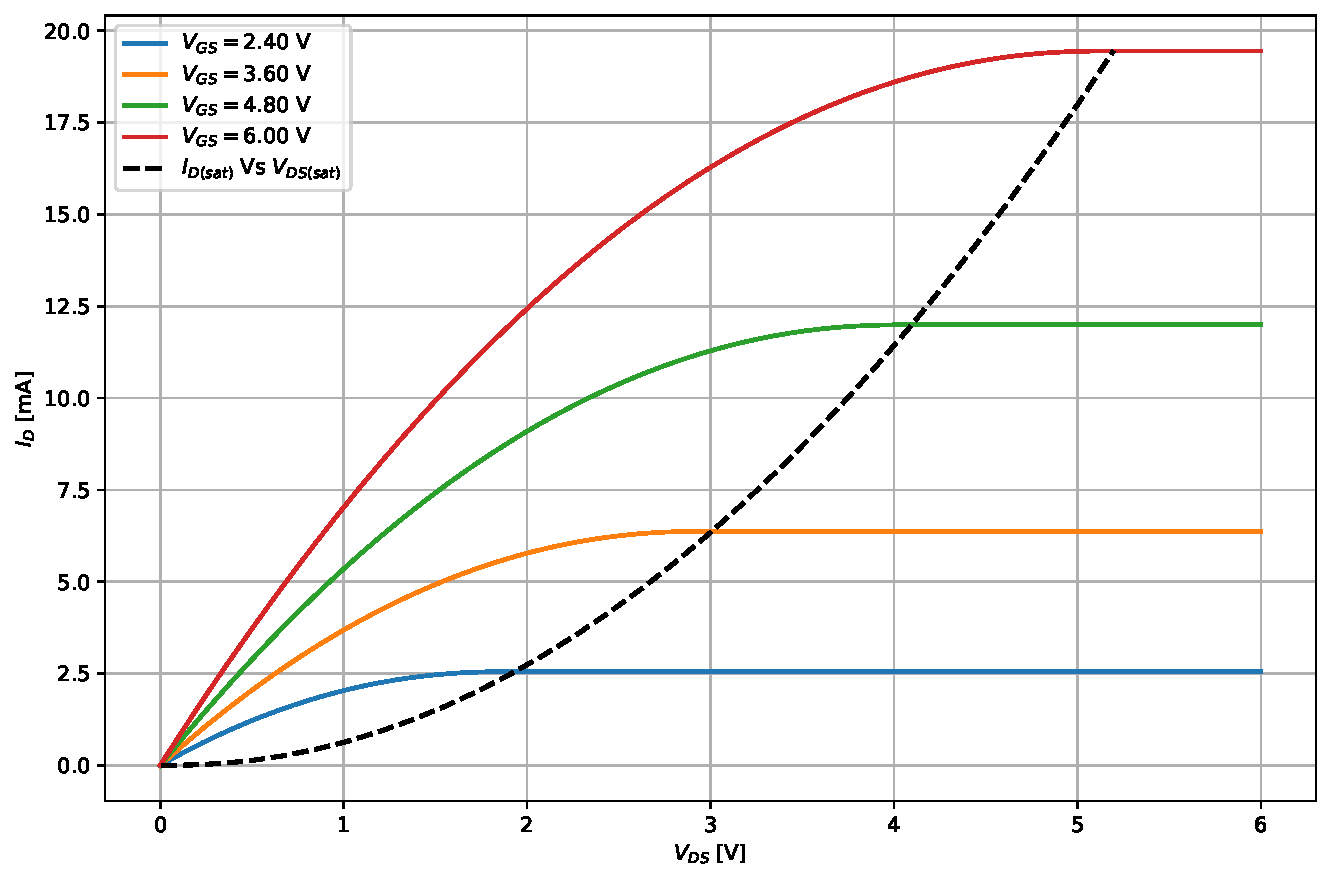
\includegraphics[width=0.7\linewidth]{res/Id_vs_vds_numerico.pdf}
    \caption{Curvas de $I_D$ contra $V_{DS}$ obtenidas numéricamente}
    \label{fig:id_vs_vds_num}
\end{figure}

\subsubsection{Aproximación cuadrática}

La aproxiamcion cuadratica nace de discriminar (\ref{eq:Id_gral}) para cada uno de los regimenes de operación, aproximando el regimen de triodo como una parábola. Se basa en las siguientes ecuaciones:

- Para $V_{GS} > V_T$ y $V_{DS} < V_{DS(sat)}$ (Régimen Lineal/Triodo):

$$I_D = \mu_n C'_{ox}\frac{W}{L} (V_{GS} - V_T -\frac{m}{2} V_{DS})V_{DS}.$$

- Para $V_{GS} > V_T$ y $V_{DS} > V_{DS(sat)}$ (Régimen de saturación):

$$I_D = \frac{\mu_n C'_{ox}}{2m}\frac{W}{L}(V_{GS} - V_T)^2.$$

- Para $V_{GS} < V_T$ (Regimen subumbral):

$$I_D = \mu_n C'_{ox}\frac{W}{L} (m-1) V_{th}^2 \exp\left(\frac{V_{GS}- V_T}{m V_{th}}\right) \left[ 1- \exp \left(-\frac{V_{DS}}{V_{th}}\right)\right].$$

Por ultimo, la curva de saturación se puede aproximar por: 

$$V_{DS(sat)} = \frac{V_{GS}-V_T}{m}.$$

$$I_D(V_{DS} = V_{DS(sat)}) \approx \mu_n C'_{ox}\frac{W}{L} \frac{1}{2m}(V_{GS} - V_T)^2.$$

A continuación el gráfico obtenido utilizando la aproximación cuadrática:

\begin{figure}[H]
    \centering
    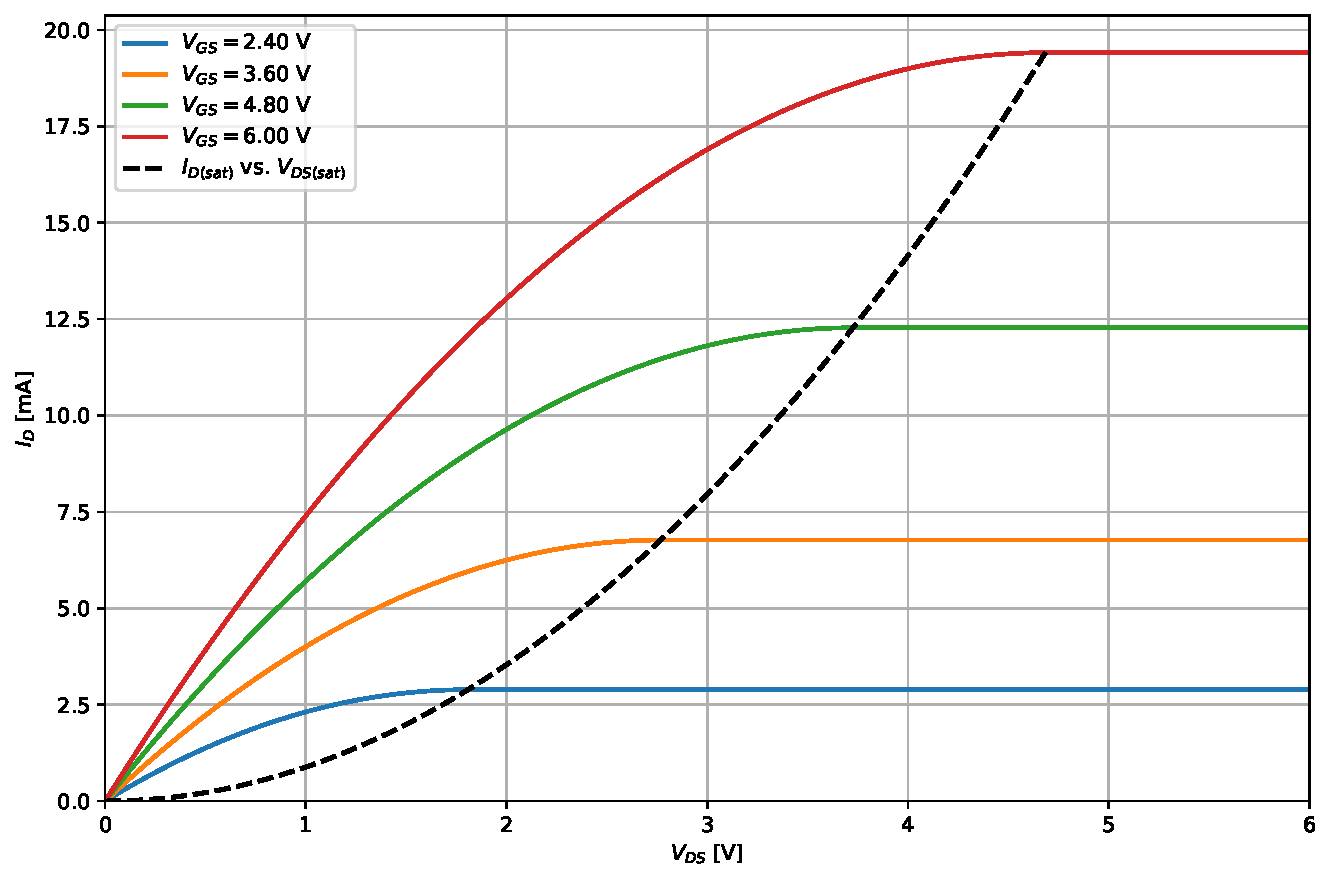
\includegraphics[width=0.7\linewidth]{res/Id_vs_vds_cuadratico.pdf}
    \caption{Curvas de $I_D$ contra $V_{DS}$ obtenidas con la aproximación cuadrática}
    \label{fig:id_vs_vds_cuad}
\end{figure}

\subsubsection{Aproximación clásica}

La aproximación clasica no es nada más que una simplificación a la aproximación cuadrática. Se utilizan las mismas ecuaciones que para la cuadrática solo que con $m = \SI{1}{}$. A continuacion el gráfico obtenido:

\begin{figure}[H]
    \centering
    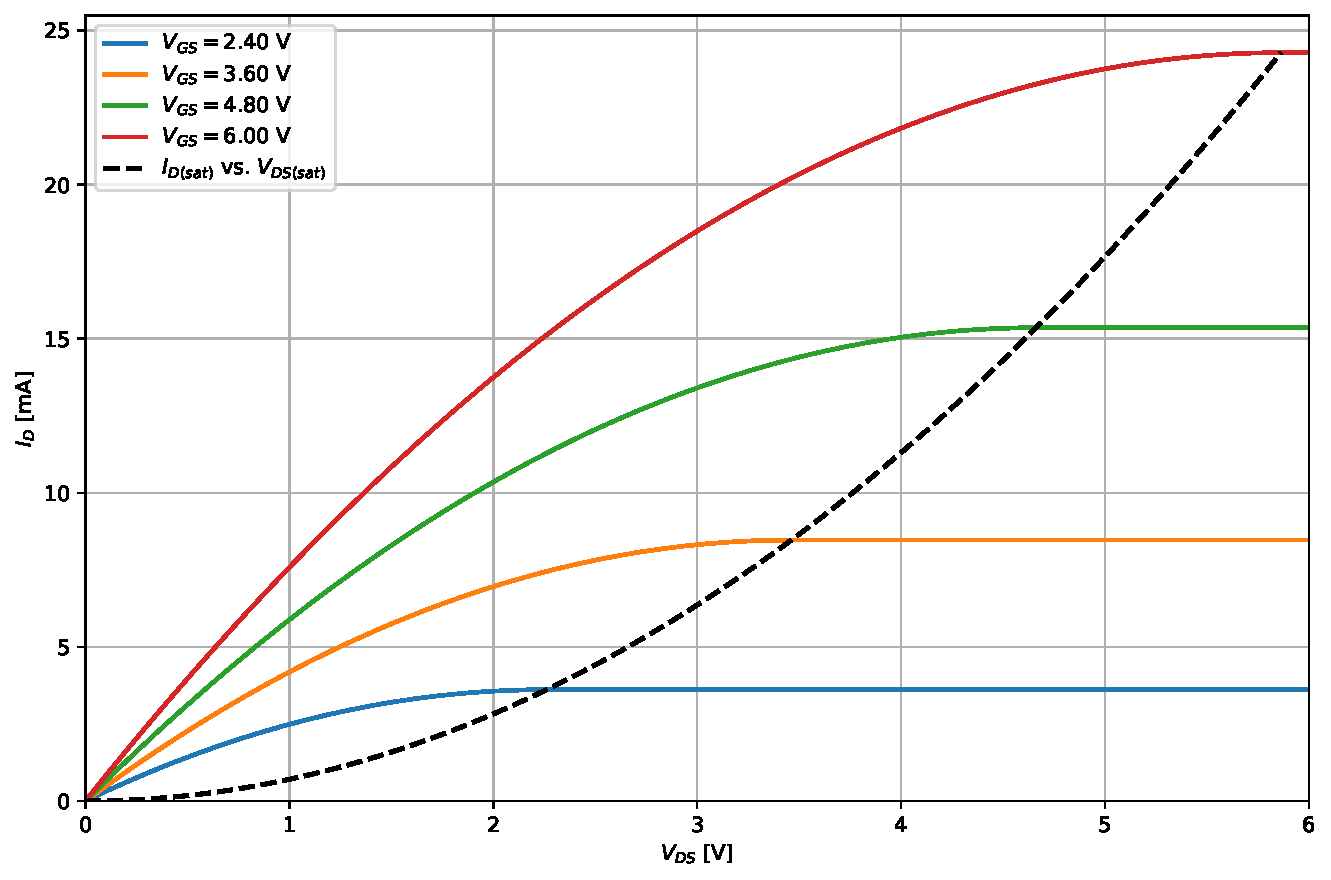
\includegraphics[width=0.7\linewidth]{res/Id_vs_vds_clasico.pdf}
    \caption{Curvas de $I_D$ contra $V_{DS}$ obtenidas con la aproximación clásica}
    \label{fig:id_vs_vds_clas}
\end{figure}

\subsubsection{Análisis y comparación de resultados}

Con el fin de realizar una mejor comparación de los tres métodos presentados, se realiza un gráfico en el que se superponen curvas obtenidas con cada uno de los métodos para un mismo valor de $V_{GS}$

\begin{figure}[H]
    \centering
    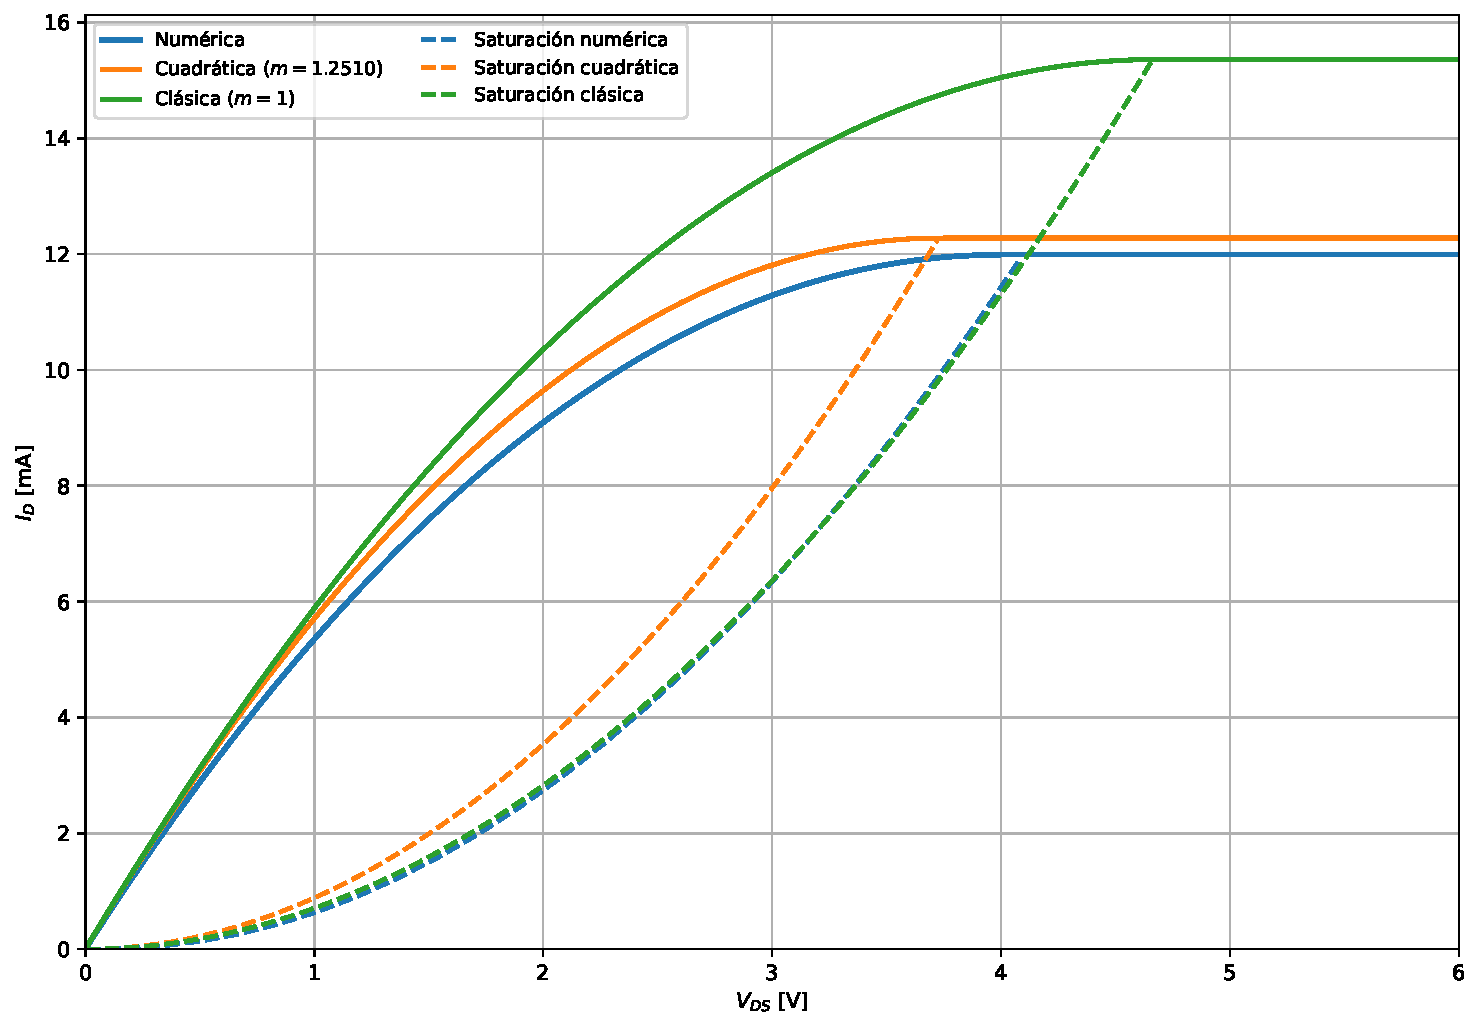
\includegraphics[width=0.7\linewidth]{res/Id_vs_vds_comparacion.pdf}
    \caption{Curvas de $I_D$ contra $V_{DS}$ con los tres métodos}
    \label{fig:id_vs_vds_comp}
\end{figure}

Se puede apreciar como la curva numérica y la cuadrática son similares, teniendo la cuadrática un error levemente mayor al $1.5\%$ en la región de saturación. La mayor discrepancia entre la aproximación cudrática y el método numérico es en la curva de saturación, se puede apreciar como el metodo numerico define la saturación en valores de tension de drain mucho más altos que la aproximación cuadrática. 

Finalmente la aproximación clásica es la que claramente más error presenta. De todas formas, la aproximación clásica deberia juzgarse por su simplicidad, ya que sin la necesidad de realizar calculos tediosos ni conocer tantos parámetros del transistor se puede tener un estimado del comportamiento, que resulta util para primeras etapas de diseño.  

\subsection{Calculo de la curva de transferencia $I_D$ vs $V_{GS}$}

Para todos los casos las ecuaciones son las mismas que en la sección anterior simplemente se realiza el barrido en $V_{GS}$ manteniendo la tensión de drain fija. Los gráficos se presentan tanto en escala lineal como en escala logaritmica, con la intención de que se puedan apreciar las corrientes de magnitudes tan distintas en los regimenes de operacion.

\subsubsection{Método numérico}

\begin{figure}[H]
    \centering
    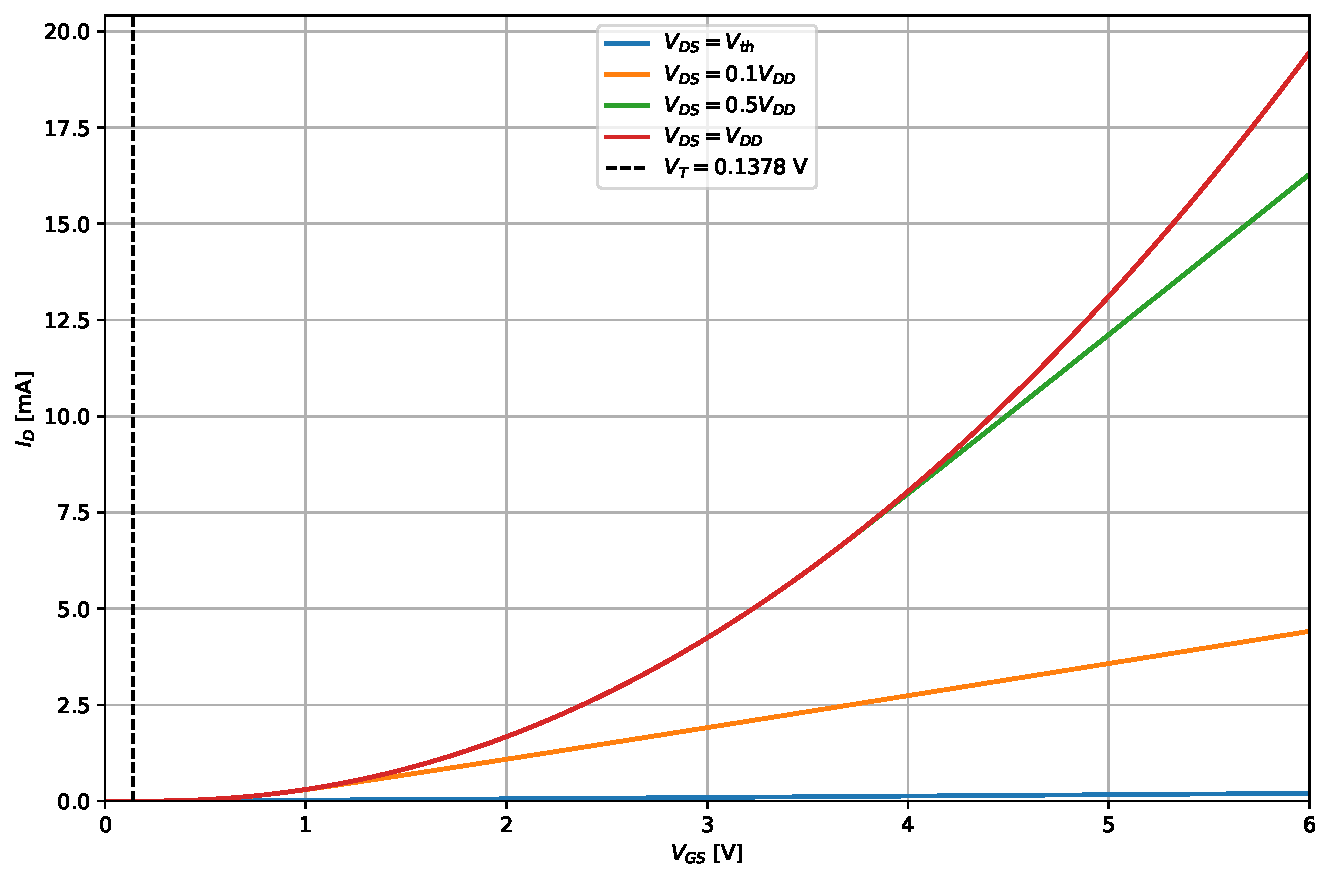
\includegraphics[width=0.7\linewidth]{res/Id_vs_vgs_numerico.pdf}
    \caption{Curvas de $I_D$ contra $V_{GS}$ obtenidas numéricamente}
    \label{fig:id_vs_vgs_num}
\end{figure}
\begin{figure}[H]
    \centering
    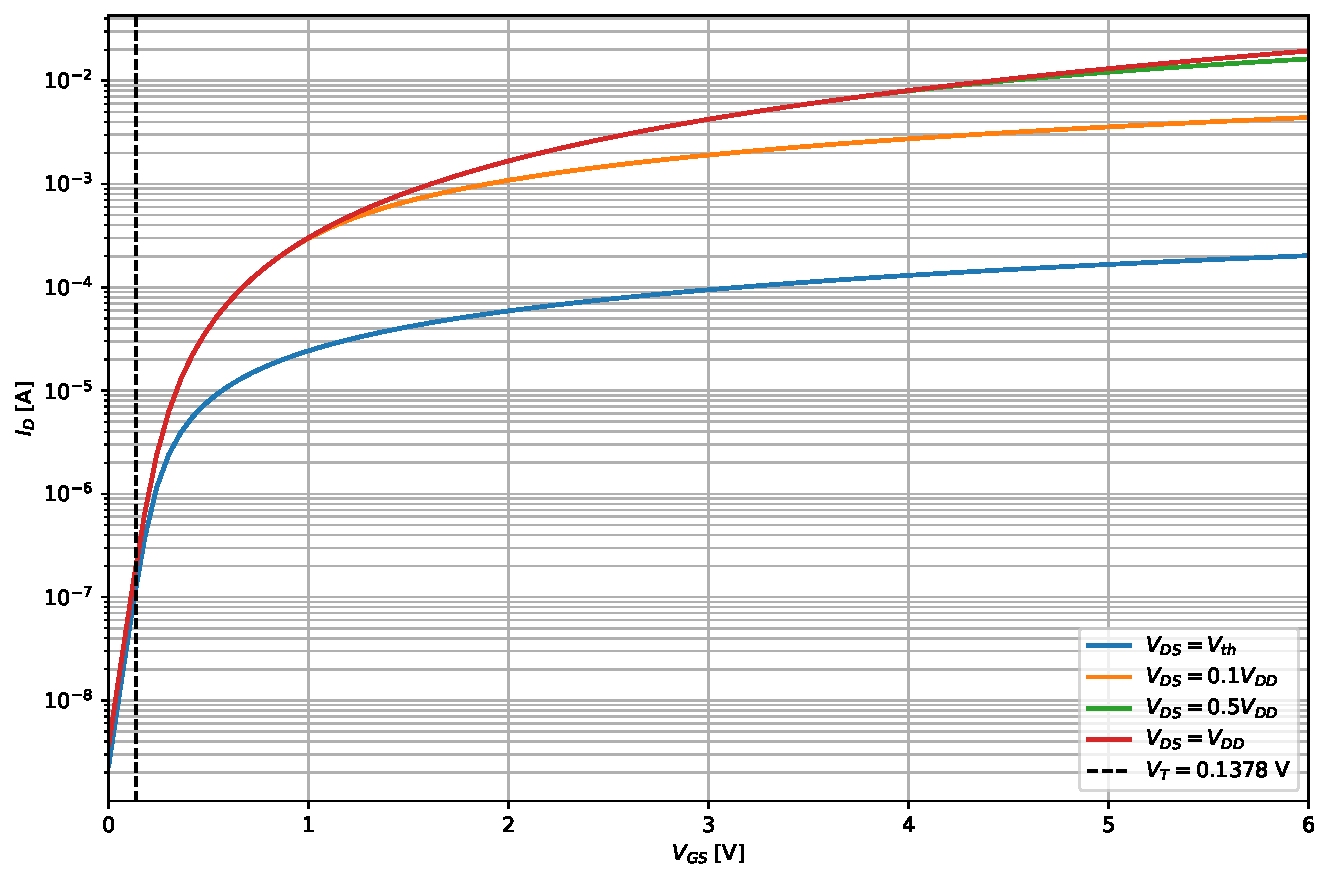
\includegraphics[width=0.7\linewidth]{res/Id_vs_vgs_numerico_log.pdf}
    \caption{Curvas de $I_D$ contra $V_{GS}$ obtenidas numéricamente en escala logarítmica}
    \label{fig:id_vs_vgs_num_log}
\end{figure}

\subsubsection{Aproximación cuadrática}

\begin{figure}[H]
    \centering
    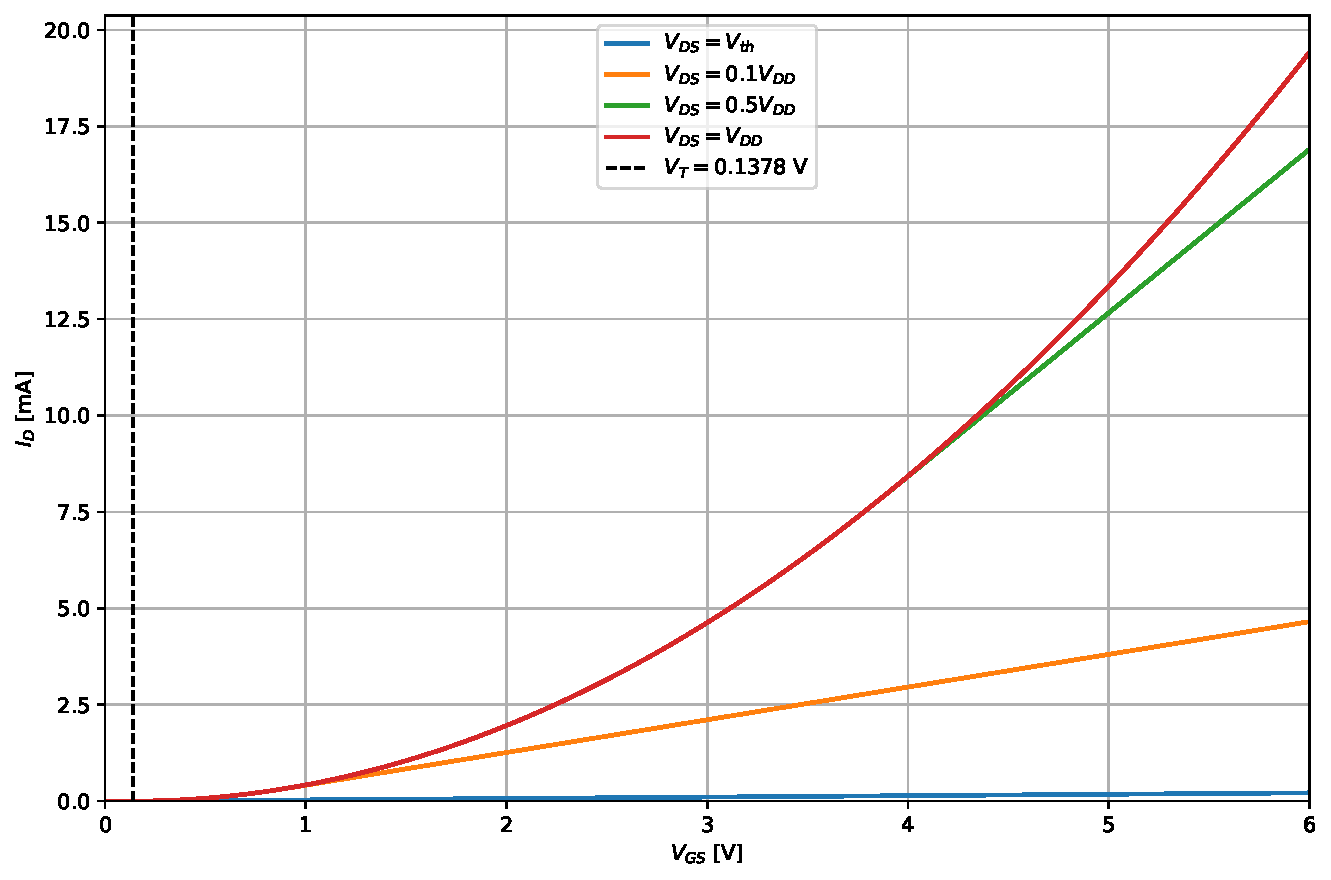
\includegraphics[width=0.7\linewidth]{res/Id_vs_vgs_cuadratico.pdf}
    \caption{Curvas de $I_D$ contra $V_{GS}$ obtenidas con la aproximación cuadrática}
    \label{fig:id_vs_vgs_cuad}
\end{figure}
\begin{figure}[H]
    \centering
    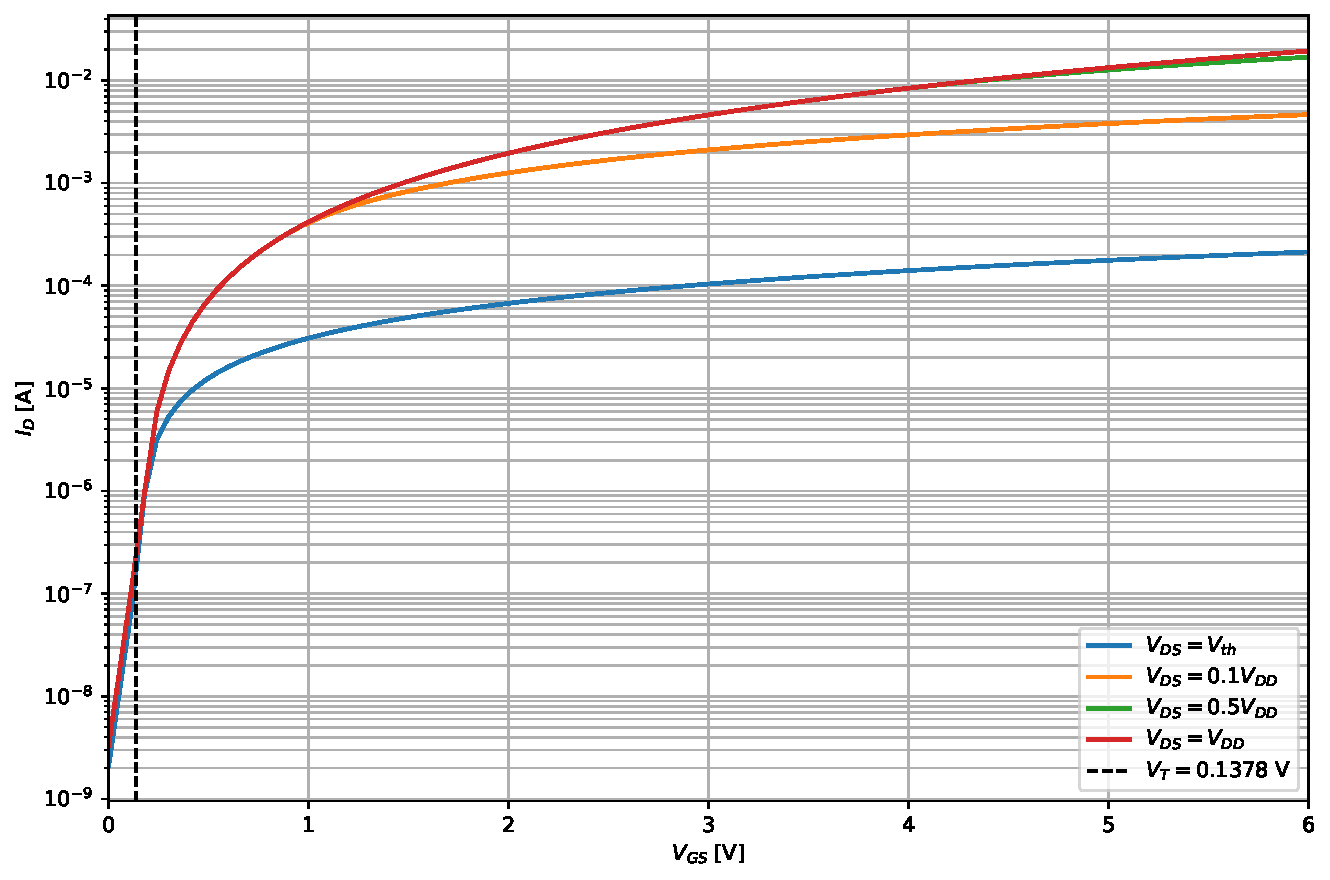
\includegraphics[width=0.7\linewidth]{res/Id_vs_vgs_cuadratico_log.pdf}
    \caption{Curvas de $I_D$ contra $V_{GS}$ obtenidas con la aproximación cuadrática en escala logarítmica}
    \label{fig:id_vs_vgs_cuad_log}
\end{figure}

\subsubsection{Aproximación clásica}

\begin{figure}[H]
    \centering
    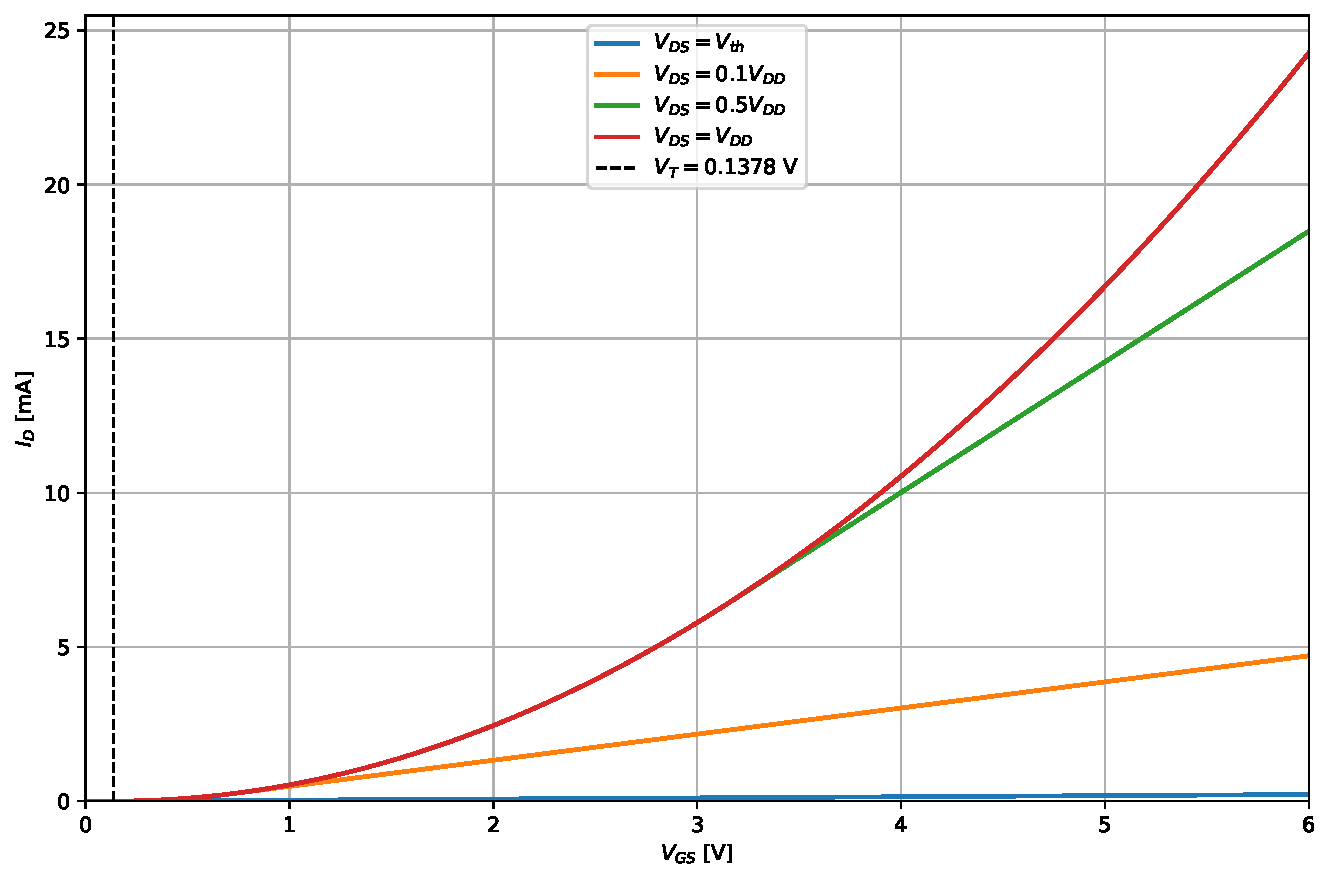
\includegraphics[width=0.7\linewidth]{res/Id_vs_vgs_clasico.pdf}
    \caption{Curvas de $I_D$ contra $V_{GS}$ obtenidas con la aproximación clásica}
    \label{fig:id_vs_vgs_clas}
\end{figure}
\begin{figure}[H]
    \centering
    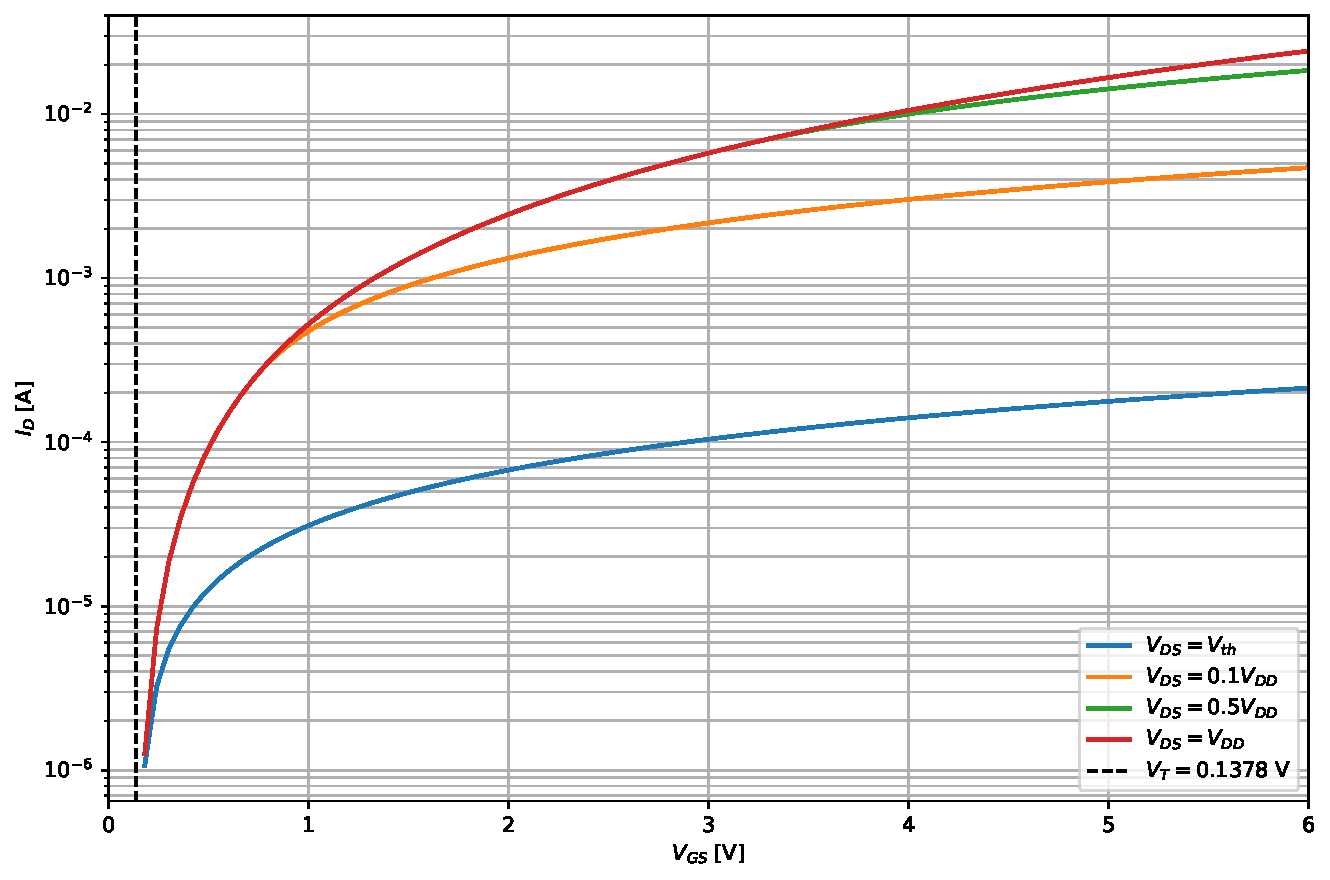
\includegraphics[width=0.7\linewidth]{res/Id_vs_vgs_clasico_log.pdf}
    \caption{Curvas de $I_D$ contra $V_{GS}$ obtenidas con la aproximación clásica en escala logarítmica}
    \label{fig:id_vs_vgs_clas_log}
\end{figure}

\subsubsection{Análisis y comparación de resultados}

De forma similar a lo ocurrido con las curvas de salida, la aproximación cuadrática y el metodo numerico se encuentran considerablemente cerca, con la curva de la aproximación clasica por encima. En el grafico con escala semilogaritmica de la \autoref{fig:id_vs_vgs_comp_log} se puede apreciar como las 3 curvas presentan un comportamiento similar en las regiones de triodo y saturación, pero en la región subumbral resulta envidente que la aproximación clasica no tiene expresión para modelar este regimen de funcionamiento. 

\begin{figure}[H]
    \centering
    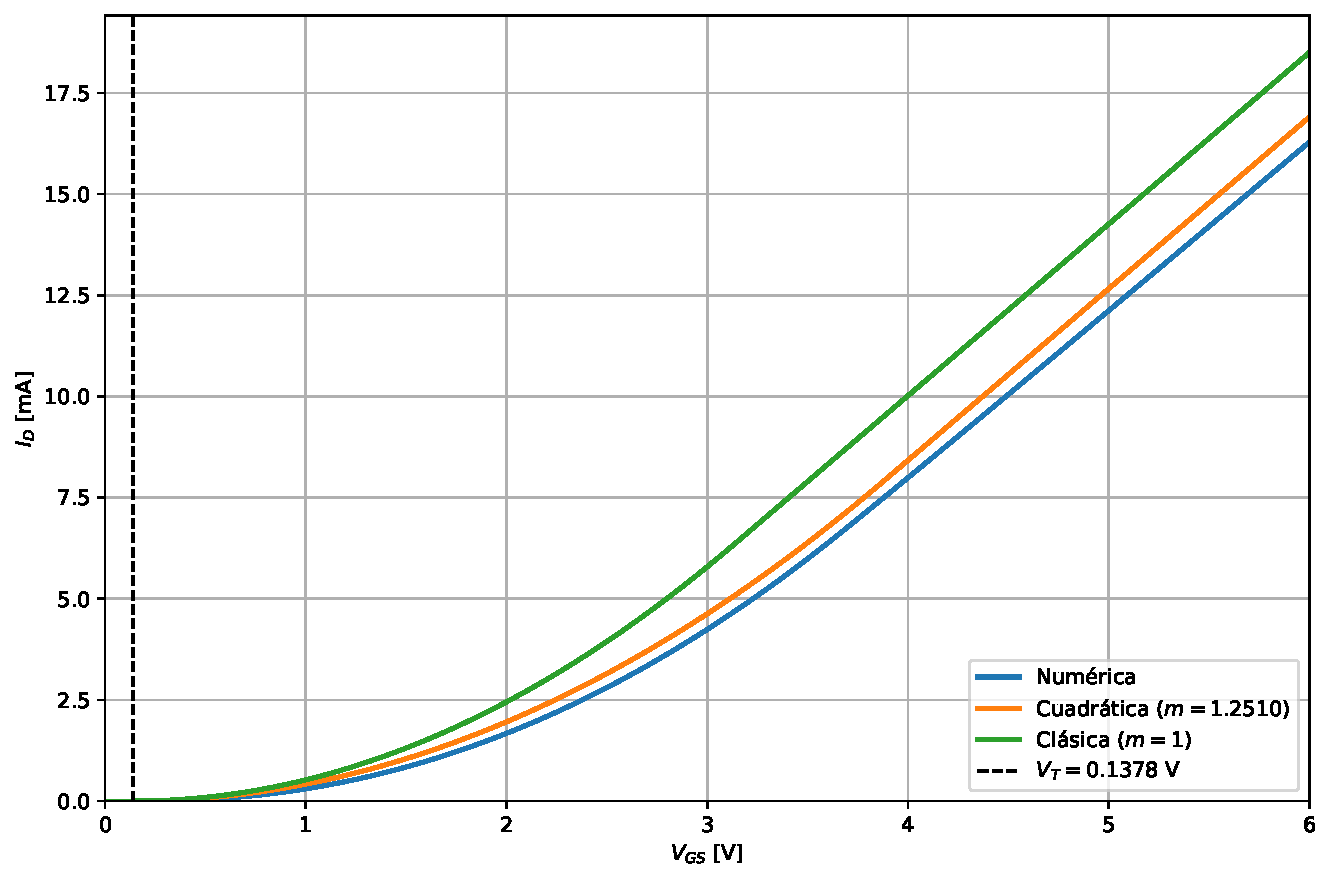
\includegraphics[width=0.7\linewidth]{res/Id_vs_vgs_comparacion.pdf}
    \caption{Curvas de $I_D$ contra $V_{GS}$ obtenidas con los tres métodos}
    \label{fig:id_vs_vgs_comp}
\end{figure}
\begin{figure}[H]
    \centering
    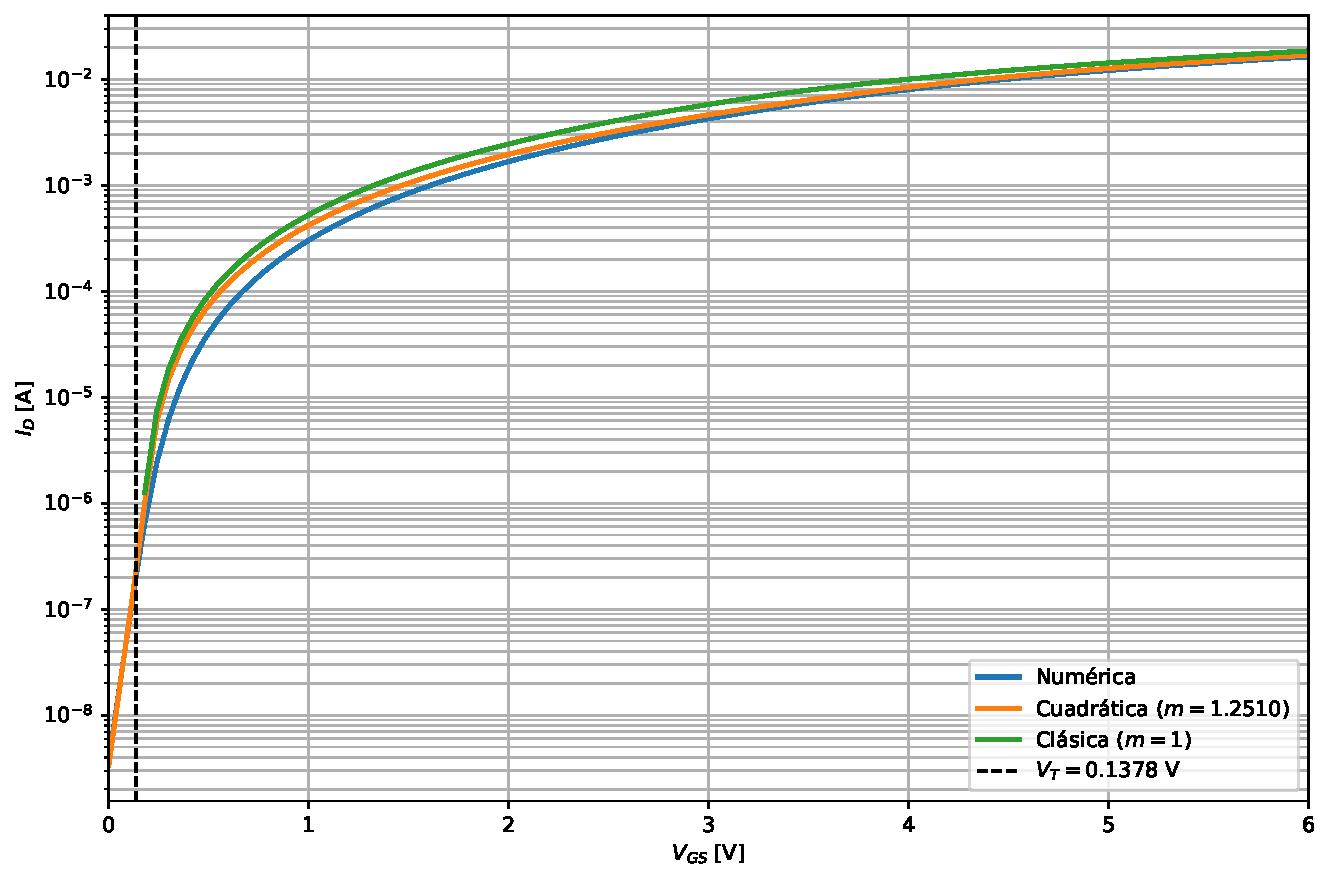
\includegraphics[width=0.7\linewidth]{res/Id_vs_vgs_comparacion_log.pdf}
    \caption{Curvas de $I_D$ contra $V_{GS}$ obtenidas con los tres métodos en escala logarítmica}
    \label{fig:id_vs_vgs_comp_log}
\end{figure}


\section{Parte II}

\subsection{Parámetros de la estructura MOS luego del escalamiento}

Partiendo de los datos asignados por la cátedra para el escalado: 

\begin{table}[H]
	\centering
	\renewcommand{\arraystretch}{1.3}
	\caption{Datos de escalado.}
	\begin{tabular}{lc}
		\toprule
		\textbf{Parámetro} & \textbf{Valor} \\
		\midrule
		$\kappa$ & \SI{12}{} \\
		$E_c$ & \SI{16}{\kilo\volt\per\centi\meter} \\
		$\alpha$ & \SI{-0.31}{} \\
		$\mu_{0}$ & \SI{1025}{\centi\meter\squared\per\volt\per\second} \\
		$E_0$ & \SI{28}{\kilo\volt\per\centi\meter} \\
		$N_{d}$ & \SI{2e20}{\per\cubic\centi\meter} \\
		\bottomrule
	\end{tabular}
\end{table}

Se escalan los parámetros fisicos de la sección anterior respecto a la tabla de escalado con campo eléctrico constante: 

- Las dimensiones del dispositivo, como $t_{ox}$, $L$, $W$, y $r_j$ se escalan por $\frac{1}{\kappa}$.

- Los dopajes se escalan por $\kappa$.

- Las tensiones se escalan por $\frac{1}{\kappa}$.

Aplicando estas reglas, se obtienen los valores escalados de la siguiente tabla:

\begin{table}[H]
	\centering
	\renewcommand{\arraystretch}{1.3}
	\caption{Datos escalados por tabla.}
	\begin{tabular}{lc}
		\toprule
		\textbf{Parámetro} & \textbf{Valor} \\
		\midrule
		$t_{ox}^*$ & \SI{2.5}{\nano\meter} \\
		$L^*$ & \SI{0.166}{\micro\meter} \\
		$W^*$ & \SI{1.66}{\micro\meter} \\
		$N_{a}^*$ & \SI{8.4e16}{\per\cubic\centi\meter} \\
		$V_{DD}^*$ & \SI{0.5}{\volt} \\
		$r_{j}^*$ & \SI{34.2}{\nano\meter} \\
		$E_{0}-E_{poly}^*$ & \SI{4.09}{\electronvolt} \\
		\bottomrule
	\end{tabular}
\end{table}

Por ultimo, con los valores escalados se recalculan todos los parámetros de la estructura MOS, de la misma forma que se hizo en la Parte I y se obtienen los valores de la siguiente tabla:

\begin{table}[H]
	\centering
	\renewcommand{\arraystretch}{1.3}
	\caption{Parámetros obtenidos post escalado.}
	\begin{tabular}{lc}
		\toprule
		\textbf{Parámetro} & \textbf{Valor} \\
		\midrule
		$\mu_{np}^*$ & \SI{762.9}{\centi\meter\squared\per\volt\per\second} \\
		$C_{ox}^*$ & \SI{3.83}{\femto\farad} \\
		$\psi_B^*$ & \SI{-0.4125}{\volt} \\
		$\phi_{\mathrm{poly}}^*$ & \SI{4.09}{\volt} \\
		$\phi_s^*$ & \SI{4.9825}{\volt} \\
		$\phi_{\mathrm{BI}(GB)}^*$ & \SI{0.9725}{\volt} \\
		$V_{FB}^*$ & \SI{-0.9725}{\volt} \\
		$\gamma^*$ & $0.121\,\sqrt{\si{\volt}}$ \\
		$V_T^*$ & \SI{-37.7}{\milli\volt} \\
		$m^*$ & \num{1.07} \\
		\bottomrule
	\end{tabular}
\end{table}

\subsection{Curva de salida $I_D$ vs. $V_{DS}$}

Con los nuevos parámetros se calculó la curva de salida utilizando la aproximaxción cuadrática y se obtuvieron las siguientes curvas: 

\begin{figure}[H]
    \centering
    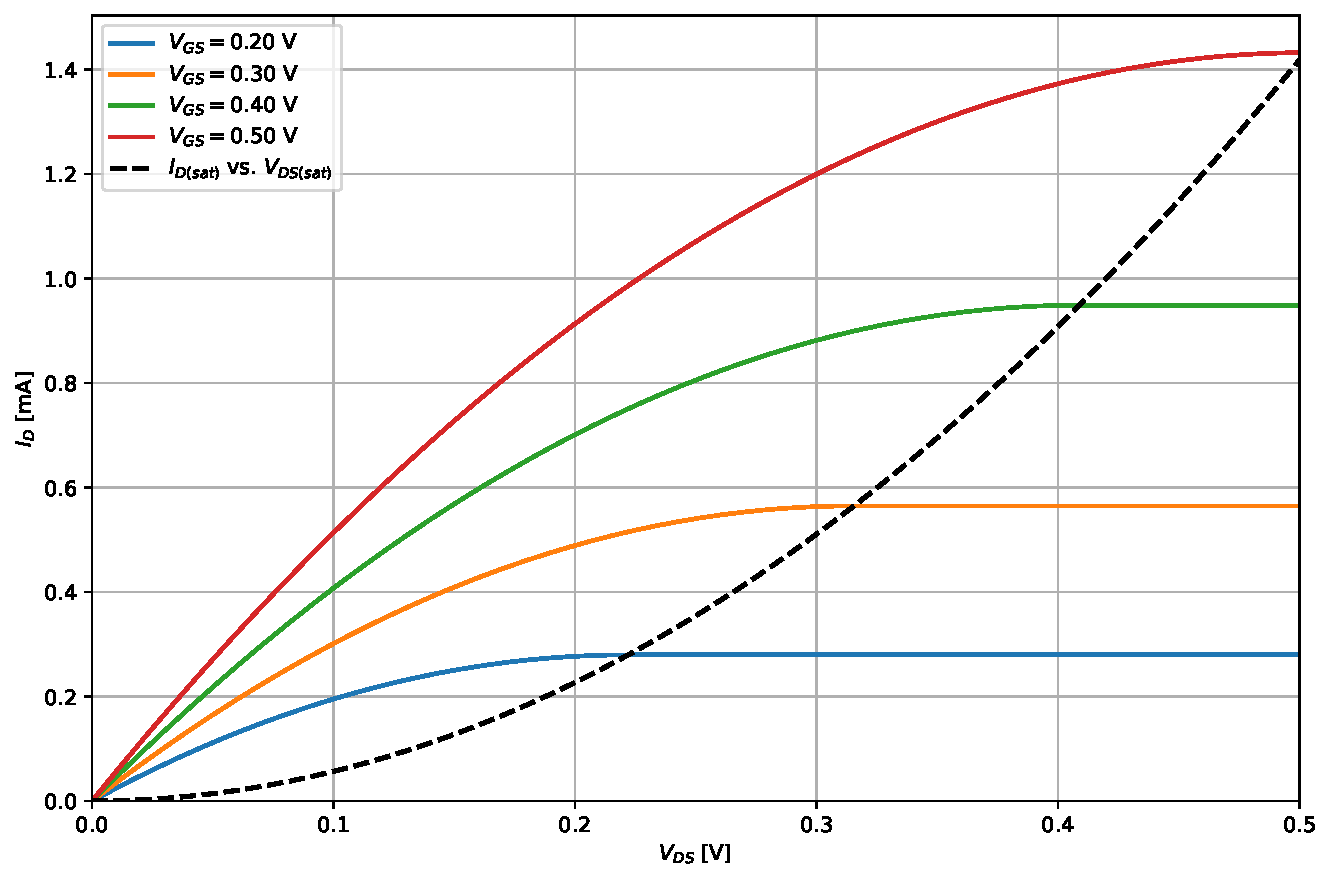
\includegraphics[width=0.7\linewidth]{res/ID_VDS_canal_corto.pdf}
    \caption{Curvas de $I_D$ contra $V_{DS}$ para el MOS canal corto}
    \label{fig:id_vs_vds_corto}
\end{figure}

Cabe destacar, que si bien las corrientes con considerablemente menores que en el caso del canal largo, las tensiones también lo son, ya que formaron aprte del escalamiento.

\subsection{Modulación del canal}

Es un fenómeno que ocurre al aumentar la tensión de drain, la region de agotamiento se extiende hacia el source y se desplaza el punto de pinch off tambien hacia el source, afectando la corriente de drain.

La corriente viene dada por: 

$$I_D = \left( \frac{L}{L-\Delta L}\right) I_{D(c)},$$

Donde

$$\Delta L = \sqrt{\frac{2 \epsilon_s}{q N_a}}\left( \sqrt{\phi_{bi_{db}}+V_{DS}} - \sqrt{\phi_{bi_{db}}+V_{DS(sat)}}\right).$$

Teniendo en cuenta la expresión de la tension de drain de saturacion:

$$V_{DS(sat)} = V_{GS} - V_T$$

se puede remplazar esta en la ecuación anterior y dejarla solamente en funcion de $V_{DS}$ y $V_{GS}$

Por ultimo, como $N_d > N_c$, se trata de un drain degenerado, por lo que se puede plantear:

\begin{equation*}
	\phi_{bi_{db}} = \frac{E_g}{2q}-\psi_B
\end{equation*}

y para los datos de este trabajo, el valor obtenido es $\phi_{bi_{db}} = \SI{0.9725}{\volt}$

A continuación el gráfico teniendo en cuenta el efecto, superpuesto a las curvas sin la presencia del efecto punteadas:

\begin{figure}[H]
    \centering
    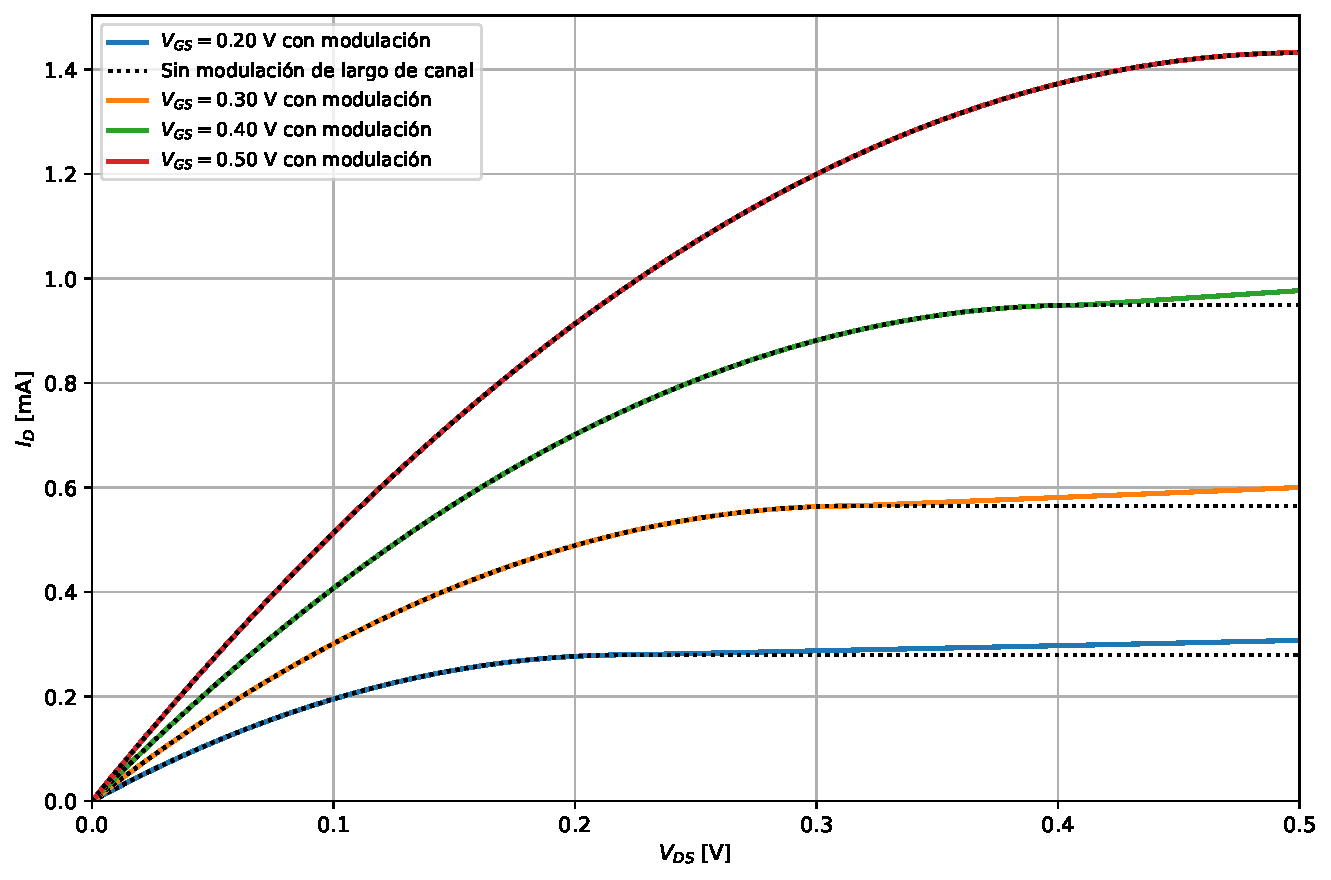
\includegraphics[width=0.7\linewidth]{res/ID_VDS_canal_corto_emlc.pdf}
    \caption{Curvas de $I_D$ contra $V_{DS}$ para el MOS canal corto con EMLC}
    \label{fig:id_vs_vds_corto_emlc}
\end{figure}

En la zona de saturacion se puede apreciar claramente como la corriente amuenta a medida que aumenta la tensión de drain, por lo que el efecto está presente en el funcionamiento. 

\subsection{Reducción de la barrera inducida por drain (DIBL)}

Sucede cuando las regiones de carga espacial de las junturas PN del dispositivo "se tocan" generando una perforacion del canal que genera una corriente entre drain y source altamente dependiente de $V_D$

Se puede calcular $x_{db0}$ de ña siguiente forma:

\begin{equation*}
	x_{db0} = \sqrt{\frac{2\epsilon_s}{q N_a} \phi_{bi,db}}
\end{equation*}

el valor obtenido es $x_{db0} = \SI{122.3}{\nano\meter}$

Tambien, la tensión de punch through reuslta:

\begin{equation*}
	V_{PT} = \frac{q N_a (L - x_{db0})^2}{2 \epsilon_s} - \phi_{bi,db}
\end{equation*}

el valor obtenido es $V_{PT} = \SI{-0.84497}{\volt}$

Por ultimo, la corriente de DIBL se puede calcular en base a la densidad de corriente que viene dada de la siguiente forma:

$$J_{D(pt)} \approx \frac{9 \epsilon_s \mu_n}{8 L^3}V_{DS}^2$$

$$I_{DIBL} = J_{D(pt)} W r_j$$

A continuacion, las curvas de salida teniendo en cuenta el fenómeno:

\begin{figure}[H]
    \centering
    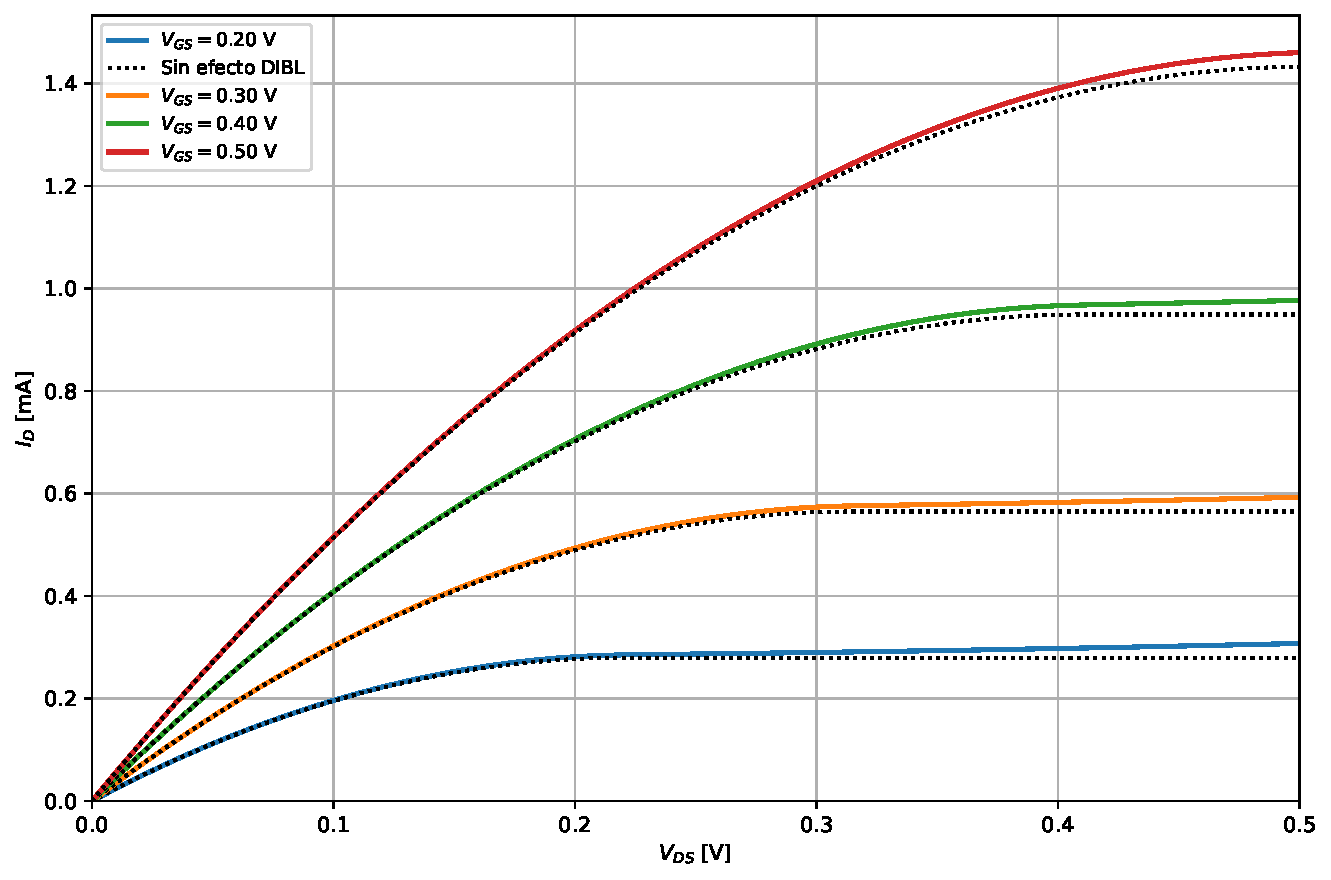
\includegraphics[width=0.7\linewidth]{res/ID_VDS_canal_corto_dibl.pdf}
    \caption{Curvas de $I_D$ contra $V_{DS}$ para el MOS canal corto con DIBL}
    \label{fig:id_vs_vds_corto_dibl}
\end{figure}

Se puede apreciar claramente un amumento de las corrientes respecto al no considerar DIBL, que resulta más evidente tanto al aumentar la tension del gate como la tensión del drain. 

\subsection{Degradación de la movilidad}

En mosfets de canal corto, cuando no satura la velocidad de portadores, la movilidad depende esencialmente del campo electrico efectivo, que viene dado por:

$$\mathscr{E}_{eff} \approx \frac{\epsilon_{ox}}{t_{ox} \epsilon_s}(V_T - V_{FB} + 2 \psi_B) + \frac{\epsilon_{ox}}{2 t_{ox} \epsilon_s} (V_{GS}-V_T)$$

y para los 4 valores de $V_{GS}$ utilizados vale:

\begin{equation*}
	\SI{304.86}{\kilo\volt\per\centi\metre}\quad
	\SI{371.533}{\kilo\volt\per\centi\metre}\quad
	\SI{438.2}{\kilo\volt\per\centi\metre}\quad
	\SI{504.867}{\kilo\volt\per\centi\metre}
\end{equation*}

Luego con estos campos y la siguiente formula se puede obtener la movilidad efectiva:

$$\mu_{eff} = \mu_0 \left( \frac{\mathscr{E}_{eff}}{E_0} \right)^\alpha$$

Para este caso vale:

\begin{equation*}
	\SI{488.955}{\centi\metre\squared\per\volt\per\second}\quad
	\SI{459.879}{\centi\metre\squared\per\volt\per\second}\quad
	\SI{436.943}{\centi\metre\squared\per\volt\per\second}\quad
	\SI{418.175}{\centi\metre\squared\per\volt\per\second}
\end{equation*}

Finalmente la corriente se calcula con la aproximación cuadrática, pero reemplazando la movilidad con la que corresponda para la tension de gate. Se obtuvo el siguiente grafico:

\begin{figure}[H]
    \centering
    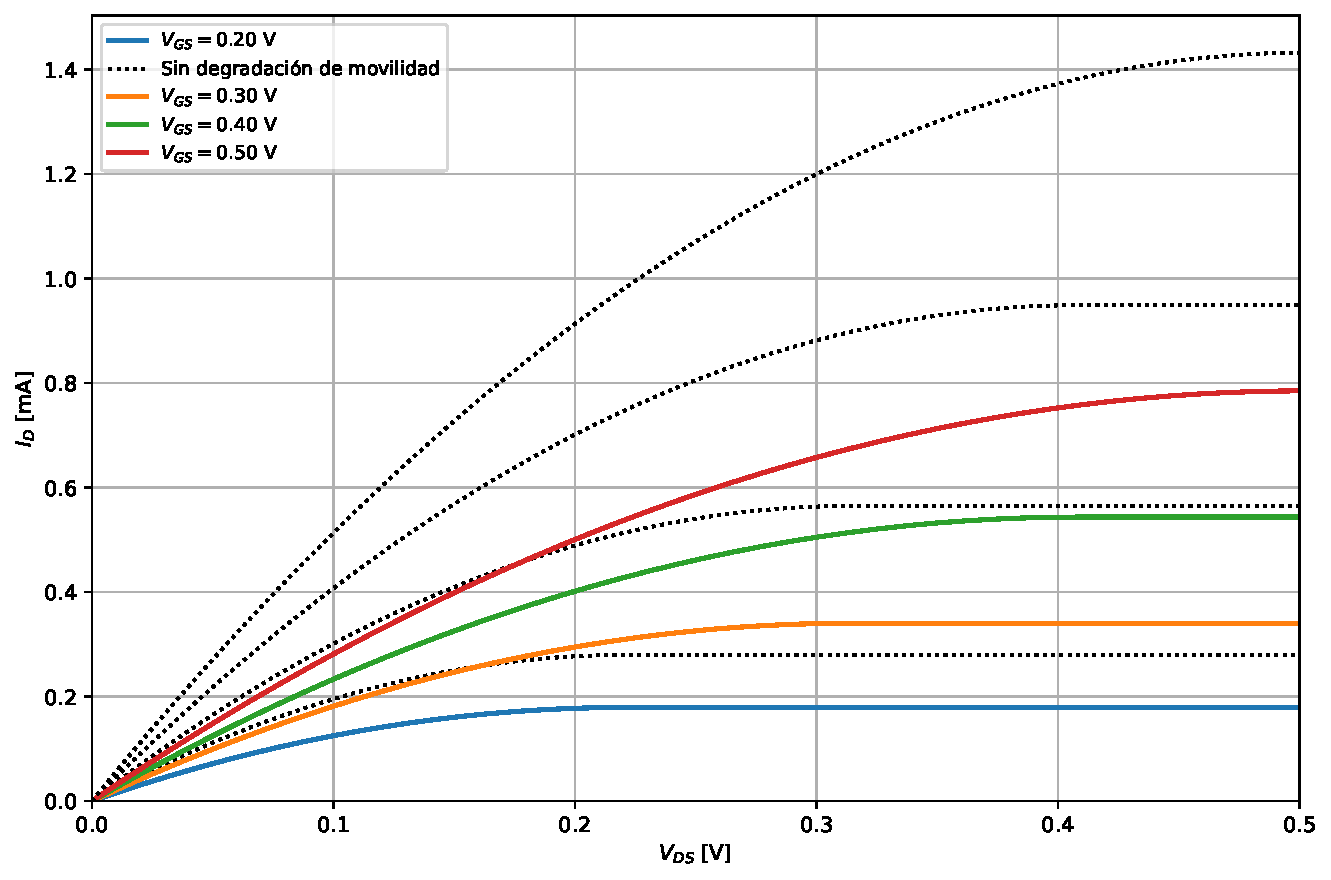
\includegraphics[width=0.7\linewidth]{res/ID_VDS_canal_corto_deg.pdf}
    \caption{Curvas de $I_D$ contra $V_{DS}$ para el MOS canal corto con movilidad degradada}
    \label{fig:id_vs_vds_corto_deg}
\end{figure}

Resulta evidente que el efecto de la degradación de la movilidad es sustancial, se puede apreciar como las corrientes disminuyeron mas de un 50\% en casi todos los casos. 

\subsection{Saturación de la velocidad de arrastre}

Se sabe que la velocidad de arrastre satura con campos elevados, y al disminuir la longitud el campo naturalmente aumenta, resultando en la saturacion de la velocidad.

La corriente del drain se puede obtener con la siguiente expresión:

$$I_D = \frac{C'_{ox} \mu_{eff}\frac{W}{L}}{1 + \frac{V_{DS}}{L E_C}}\left( V_{GS} - V_T -\frac{m}{2}V_{DS}\right)V_{DS}$$

A continuación el grafico obtenido teniendo en cuenta la saturación de velocidad, cabe destacar que en este caso se compara con las curvas que presentan degradación de la movilidad.

\begin{figure}[H]
    \centering
    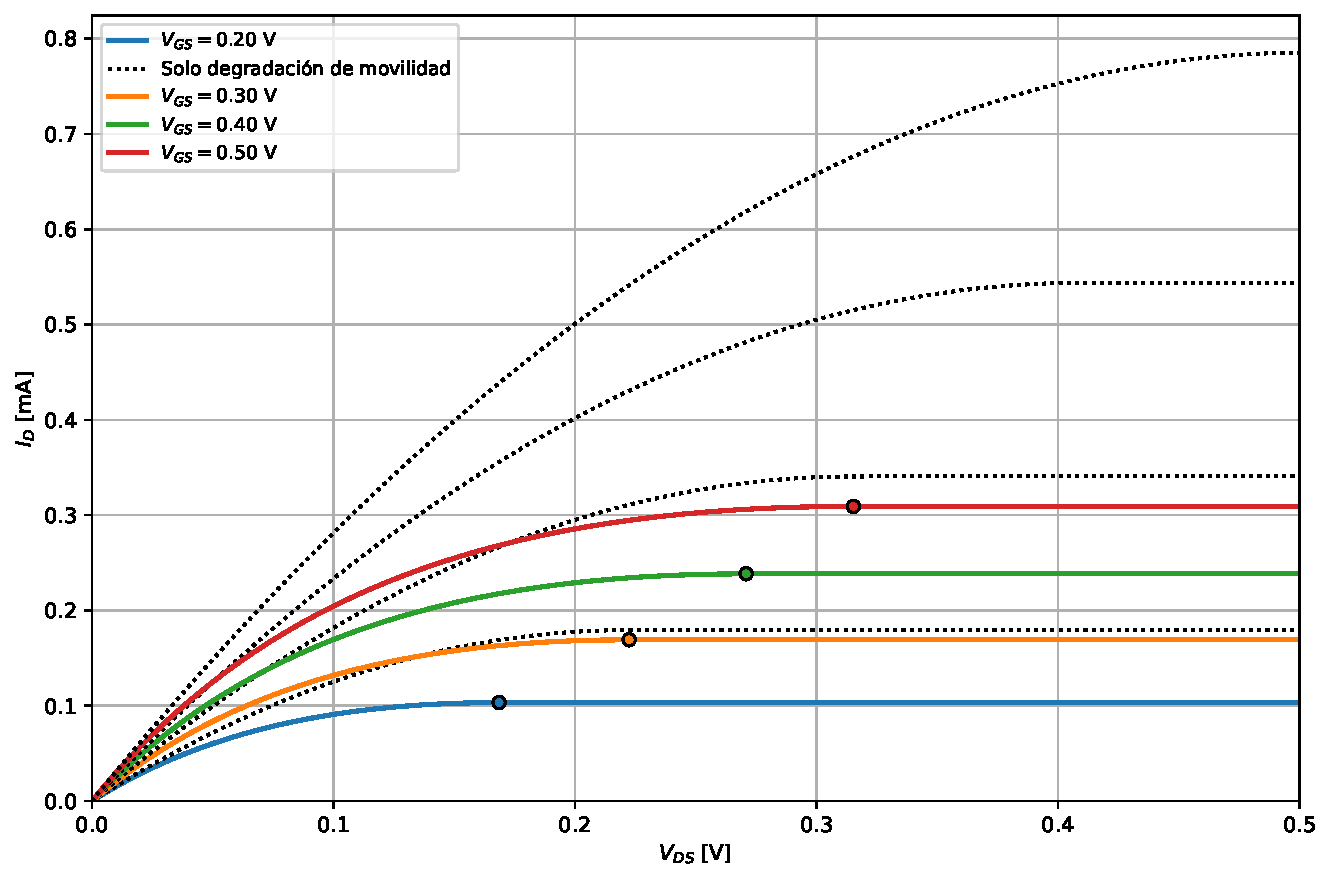
\includegraphics[width=0.7\linewidth]{res/ID_VDS_canal_corto_sat.pdf}
    \caption{Curvas de $I_D$ contra $V_{DS}$ para el MOS canal corto con saturación de velocidad}
    \label{fig:id_vs_vds_corto_sat}
\end{figure}

Resulta evidente que la velocidad está saturando, ya que las corrientes disminuyeron sustancialmente respecto a las de degradación de la movilidad.

\subsection{Curva de salida de MOSFET canal corto}

A continuacion un grafico con las curvas de salida del MOSFET canal corto teniendo en cuenta todos los efectos.

\begin{figure}[H]
	\centering
	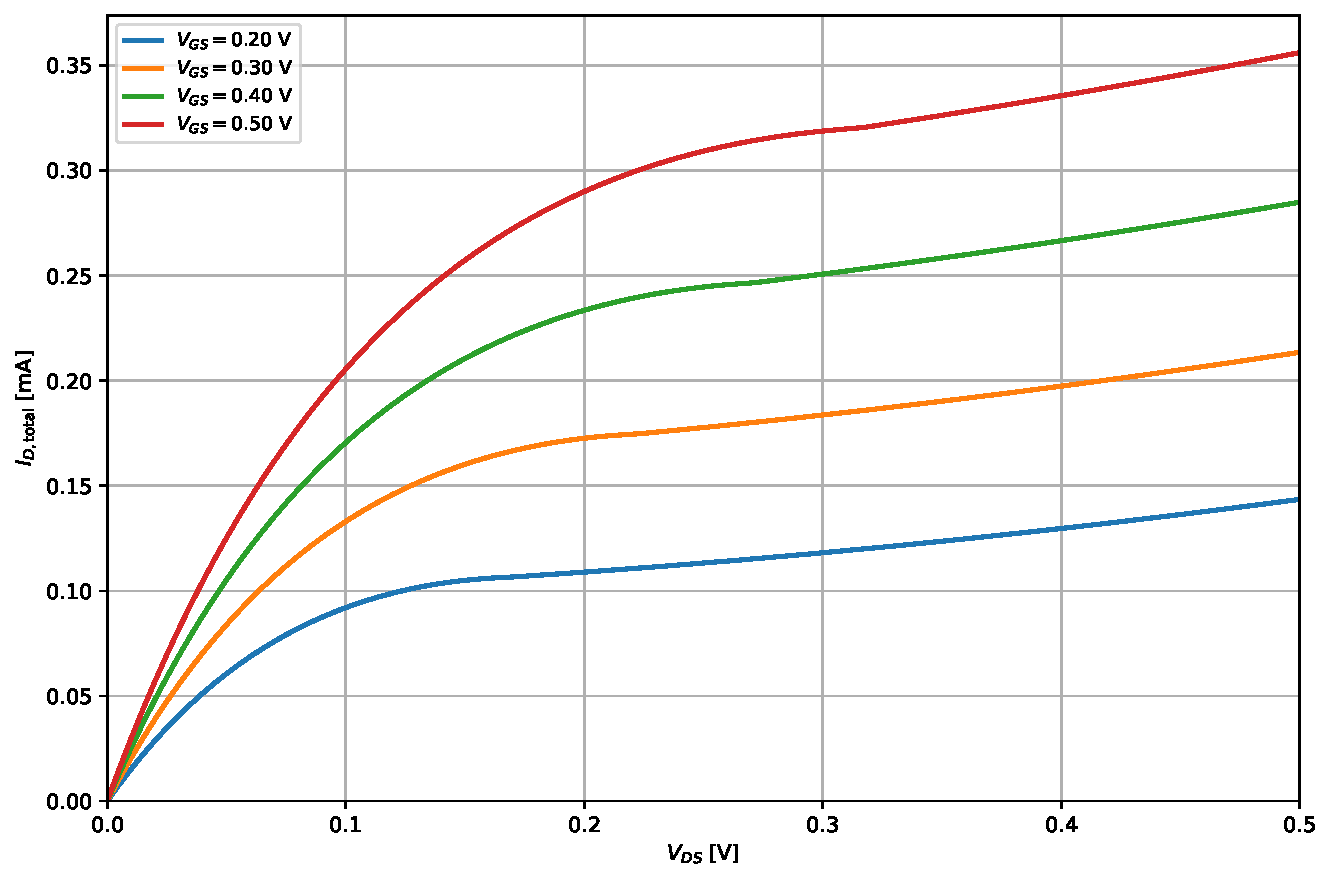
\includegraphics[width=0.7\linewidth]{res/ID_VDS_canal_corto_todos.pdf}
	\caption{Curvas de $I_D$ contra $V_{DS}$ para el MOS canal corto con todos los efectos}
	\label{fig:id_vs_vds_corto_todos}
\end{figure}

\subsection{Análisis de resultados}
	Observando la \autoref{fig:id_vs_vds_corto_todos} y comparandola con la \autoref{fig:id_vs_vds_corto}, lo que primero llama la atencíon es la diferencia en las magnitudes, las de la ultima se encuentran casi que un orden de magnitud por debajo de las de la primera. Se atribuye tal cambio al efecto combinado de la degradacion de la movilidad y la saturación de la velocidad de arrastre. 
	
	Luego de apreciar las magnitudes, lo próximo considerable es el aumento de la conrriente a medida que aumenta la tensión de drain en saturación. Esto se atribuye al efecto combinado de el DIBL y el EMLC, que quiza por su cuenta ninguno genera cambios alarmantes, pero combinados presentan una gran alteración del comportamiento en saturación. 
	
	Sin duda el efecto que más modificó la respuesta respecto a la que no consideraba ningún efecto es la saturación de velocidad de arrastre.

	Respecto al transistor de canal corto obtenido, para evaluar su calidad se puede volver a la definicion de transistor dada al principio del informe, de un transistor se espera poder controlar la corriente entre sus terminales. Si se es estricto con esa postura, se puede afirmar que el transistor cumple su trabajo, existe una clara relación entre la tension en el gate y la corriente de salida. Sin embargo, si se hace más enfasis en los usos tipicos de un transistor, uno de ellos es el uso como aplificador, donde se precisa que el comportamiento en el regimen de triodo sea lo más lineal posible. En este ultimo caso el transistor no sería el adecuado. 
	
	El transistor podría ser mejor en multiples aspectos, en especial en los comportamientos de canal corto, pero aun asi se le puede dar uso en tareas que no requieran tanta linealidad. 



\section{Conclusiones}

Durante el desarrollo del trabajo se logró caracterizar los parámetros del transistor para despues utilizar metodos y aproximaciones para modelar su comportamiento con exito. 

Luego de escalar los parámetros fisicos y recalcular los que correspondían, se analizaron los efectos de canal corto y se caracterizó a cada uno en la curva de transferencia. 

En todos los casos los resultados fueron coeherentes con lo esperado, y las respuestas gráficas obtenidas reflejaron las caracteristicas esperadas.

\pagebreak

\appendix

\section{Código utilizado}

Aclaración: El código se genero con la intención de ser utilizado en un notebook de Python, y se utilizo en el mismo, por lo que puede que los bloques no sigan el orden de ejecución en el que están presentados.

\subsection{Parte I}
\begin{verbatim}
import numpy as np
import matplotlib.pyplot as plt

from scipy.optimize import brentq


# ============================================================
# PARÁMETROS DEL DISPOSITIVO
# Usar unidades consistentes, en este ejemplo se usa SI.
# ============================================================

q = 1.602176634e-19           # C
Vth = 0.025875                 # V

Na = 7.0e15                   # 1/cm^3
ni = 1.0e10                   # 1/cm^3

epsilon_0 = 88.541878128e-15  # F/cm
epsilon_si = 11.7 * epsilon_0 # F/cm

Cox = 115.05e-9                 # F/cm^2

VFB = -0.9082                    # V

VDD = 6

PHI_B = -0.3482

VT = 0.1378

# ============================================================
# VALORES A BARRER
# ============================================================

Vds_values = np.linspace(0.0, VDD, 151)

Vgs_values = [
    0.4*VDD,
    0.6*VDD,
    0.8*VDD,
    VDD
]


# Intervalo de búsqueda de psi_sd
psi_min = -0.5
psi_max = 10

# Resolución del barrido usado para encontrar cambios de signo
number_of_scan_points = 5000

# Valor esperado para psi_sd al comienzo de cada curva
psi_initial_hint = 0.5


# ============================================================
# CAMPO ELÉCTRICO AL CUADRADO
# ============================================================

def electric_field_squared(psi_sd, Vds):
    """
    Calcula E_s^2 según la primera ecuación.
    """

    normalized_psi = psi_sd / Vth
    normalized_vds = -Vds / Vth

    # Protección contra overflow en las exponenciales
    normalized_psi = np.clip(
        normalized_psi,
        -700.0,
        700.0
    )

    normalized_vds = np.clip(
        normalized_vds,
        -700.0,
        700.0
    )

    majority_carrier_term = (
        np.exp(-normalized_psi)
        + normalized_psi
        - 1.0
    )

    minority_carrier_term = (
        np.exp(normalized_vds)
        * np.expm1(normalized_psi)
        - normalized_psi
    )

    bracket = (
        majority_carrier_term
        + (ni / Na) ** 2 * minority_carrier_term
    )

    return (
        2.0 * q * Vth * Na / epsilon_si
    ) * bracket


# ============================================================
# CARGA SUPERFICIAL
# ============================================================

def surface_charge(psi_sd, Vgs):
    """
    Q'_s = -Cox(Vgs - VFB - psi_sd)
    """

    return -Cox * (Vgs - VFB - psi_sd)


# ============================================================
# ECUACIÓN RESIDUAL
# ============================================================

def residual(psi_sd, Vds, Vgs):
    """
    Se resuelve:

        Q'_s^2 - epsilon_si^2 E_s^2 = 0

    Se supone que la segunda ecuación correcta es:

        E_s^2 = (Q'_s / epsilon_si)^2
    """

    Qs = surface_charge(psi_sd, Vgs)
    E2 = electric_field_squared(psi_sd, Vds)

    return Qs**2 - epsilon_si**2 * E2


# ============================================================
# ENCONTRAR TODAS LAS RAÍCES
# ============================================================

def find_all_roots(Vds, Vgs):
    """
    Encuentra todas las raíces dentro de:
        psi_min <= psi_sd <= psi_max
    """

    psi_grid = np.linspace(
        psi_min,
        psi_max,
        number_of_scan_points
    )

    residual_values = np.array([
        residual(psi, Vds, Vgs)
        for psi in psi_grid
    ])

    roots = []

    for index in range(len(psi_grid) - 1):
        psi_left = psi_grid[index]
        psi_right = psi_grid[index + 1]

        residual_left = residual_values[index]
        residual_right = residual_values[index + 1]

        if not (
            np.isfinite(residual_left)
            and np.isfinite(residual_right)
        ):
            continue

        if residual_left == 0.0:
            roots.append(psi_left)

        elif residual_left * residual_right < 0.0:
            root = brentq(
                lambda psi: residual(
                    psi,
                    Vds,
                    Vgs
                ),
                psi_left,
                psi_right,
                xtol=1e-12,
                rtol=1e-12,
                maxiter=200
            )

            roots.append(root)

    # Eliminar raíces repetidas
    roots = sorted(roots)
    unique_roots = []

    for root in roots:
        if (
            len(unique_roots) == 0
            or abs(root - unique_roots[-1]) > 1e-7
        ):
            unique_roots.append(root)

    return np.array(unique_roots)


# ============================================================
# CALCULAR UNA CURVA COMPLETA PARA UN Vgs
# ============================================================

def calculate_psi_curve(Vds_array, Vgs):
    """
    Sigue una misma rama de soluciones.

    Para el primer Vds elige la raíz más cercana a
    psi_initial_hint.

    Para los siguientes valores de Vds elige la raíz más
    cercana a la solución anterior.
    """

    psi_results = np.full(
        len(Vds_array),
        np.nan
    )

    previous_psi = None

    for index, Vds in enumerate(Vds_array):
        roots = find_all_roots(Vds, Vgs)

        # Opcional:
        # conservar solamente soluciones psi_sd >= 0
        roots = roots[roots >= 0.0]

        if len(roots) == 0:
            print(
                f"No se encontró solución para "
                f"Vgs = {Vgs:.3f} V, "
                f"Vds = {Vds:.3f} V"
            )
            continue

        if previous_psi is None:
            selected_root_index = np.argmin(
                np.abs(roots - psi_initial_hint)
            )
        else:
            selected_root_index = np.argmin(
                np.abs(roots - previous_psi)
            )

        selected_root = roots[selected_root_index]

        psi_results[index] = selected_root
        previous_psi = selected_root

    return psi_results
\end{verbatim}

\begin{verbatim}
    # ============================================================
# CALCULAR Y GRAFICAR TODAS LAS CURVAS
# ============================================================

plt.figure(figsize=(9, 6))

for Vgs in Vgs_values:
    psi_sd_values = calculate_psi_curve(
        Vds_values,
        Vgs
    )

    plt.plot(
        Vds_values,
        psi_sd_values,
        linewidth=1.8,
        label=rf"$V_{{gs}}={Vgs:.2f}\ \mathrm{{V}}$"
    )
plt.plot(
    Vds_values,
    Vds_values - 2* PHI_B,
    color="black",
    linestyle="--",
    linewidth=2,
    label=r"$V_{DS} - 2\phi_B$"
)



plt.xlabel(r"$V_{ds}$ [V]")
plt.ylabel(r"$\psi_{sd}$ [V]")


plt.grid(True)
plt.legend()
plt.tight_layout()

plt.savefig(
"phisd_vs_vds.pdf",
format="pdf",
bbox_inches="tight"
)

plt.show()
\end{verbatim}

\begin{verbatim}
    # ============================================================
# PARÁMETROS ADICIONALES PARA CALCULAR ID
# ============================================================

mu_n = 1228.35   # Movilidad electrónica [cm^2 / (V s)]
W = 20e-4        # Ancho del canal [cm]
L = 2e-4         # Longitud del canal [cm]


# ============================================================
# EXPRESIÓN EVALUADA EN CADA POTENCIAL SUPERFICIAL
# ============================================================

def current_primitive(psi_s, Vgs):
    """
    Evalúa la expresión entre llaves de la ecuación de ID.

    En esta función:
        Vth = tensión térmica

    psi_s puede ser un escalar o un array de NumPy.
    """

    psi_s = np.asarray(psi_s, dtype=float)

    result = np.full_like(
        psi_s,
        np.nan,
        dtype=float
    )

    # La expresión contiene sqrt(psi_s) y psi_s^(3/2).
    valid = np.isfinite(psi_s) & (psi_s >= 0.0)

    psi = psi_s[valid]

    depletion_factor = np.sqrt(
        2.0 * epsilon_si * q * Na
    )

    result[valid] = (
        # Vth es la tensión térmica
        Cox * (Vgs - VFB + Vth) * psi

        - 0.5 * Cox * psi**2

        - (2.0 / 3.0)
        * depletion_factor
        * psi**1.5

        + Vth
        * depletion_factor
        * np.sqrt(psi)
    )

    return result


# ============================================================
# CALCULAR ID PARA UN VGS Y UN ARRAY DE VDS
# ============================================================

def calculate_id_curve(Vds_array, Vgs):
    """
    Calcula ID para un conjunto de valores de VDS
    y un único valor de VGS.

    1. Calcula psi_sd(VDS) mediante calculate_psi_curve().
    2. Obtiene psi_ss como psi_sd para VDS = 0.
    3. Calcula:

       ID = mu_n * W/L *
            [F(psi_sd, Vgs) - F(psi_ss, Vgs)]

    Devuelve:
        Id_values
        psi_sd_values
        psi_ss
    """

    Vds_array = np.asarray(
        Vds_array,
        dtype=float
    )

    # Buscar la posición correspondiente a VDS = 0.
    zero_indices = np.where(
        np.isclose(
            Vds_array,
            0.0,
            atol=1e-14,
            rtol=0.0
        )
    )[0]

    if len(zero_indices) == 0:
        raise ValueError(
            "Vds_array debe contener VDS = 0 para "
            "determinar psi_ss."
        )

    # Potencial superficial del drenaje para cada VDS.
    psi_sd_values = calculate_psi_curve(
        Vds_array,
        Vgs
    )

    # Para el mismo VGS, psi_ss es psi_sd evaluado en VDS = 0.
    zero_index = zero_indices[0]
    psi_ss = psi_sd_values[zero_index]

    if not np.isfinite(psi_ss):
        raise ValueError(
            f"No se pudo calcular psi_ss para "
            f"VGS = {Vgs:.6f} V."
        )

    # Evaluación en el límite superior.
    upper_limit = current_primitive(
        psi_sd_values,
        Vgs
    )

    # Evaluación en el límite inferior.
    lower_limit = current_primitive(
        psi_ss,
        Vgs
    )

    Id_values = (
        mu_n
        * (W / L)
        * (
            upper_limit
            - lower_limit
        )
    )

    return Id_values, psi_sd_values, psi_ss
\end{verbatim}

\begin{verbatim}
    # ============================================================
# CURVA ID(sat) VS VDS(sat)
# Reutilizando calculate_id_curve()
# ============================================================

Vt = 0.1378  # Tensión de threshold [V]

# La consigna exige al menos 20 valores
Vgs_sat_values = np.linspace(
    Vt,
    VDD,
    30
)


def saturation_residual(psi_sd, Vgs):
    """
    Condición de intersección:

        psi_sd = VDS(sat) - 2*PHI_B

    Por lo tanto:

        VDS(sat) = psi_sd + 2*PHI_B
    """

    Vds_sat = psi_sd - 2.0 * PHI_B

    return residual(
        psi_sd,
        Vds_sat,
        Vgs
    )


def find_saturation_point(Vgs, previous_psi_sat=None):
    """
    Encuentra directamente la intersección sin calcular
    toda la curva psi_sd(VDS).
    """

    # Asegura VDS(sat) >= 0:
    #
    # psi_sd + 2*PHI_B >= 0
    psi_lower = max(
        0.0,
        -2.0 * PHI_B
    )

    psi_scan = np.linspace(
        psi_lower,
        psi_max,
        400
    )

    residual_scan = saturation_residual(
        psi_scan,
        Vgs
    )

    valid_pairs = (
        np.isfinite(residual_scan[:-1])
        & np.isfinite(residual_scan[1:])
    )

    crossing_indices = np.where(
        valid_pairs
        & (
            residual_scan[:-1]
            * residual_scan[1:]
            < 0.0
        )
    )[0]

    if len(crossing_indices) == 0:
        return np.nan, np.nan

    roots = []

    for index in crossing_indices:

        psi_left = psi_scan[index]
        psi_right = psi_scan[index + 1]

        root = brentq(
            lambda psi: saturation_residual(
                psi,
                Vgs
            ),
            psi_left,
            psi_right,
            xtol=1e-12,
            rtol=1e-10,
            maxiter=100
        )

        roots.append(root)

    roots = np.asarray(roots)

    # Para el primer VGS elegimos la raíz cercana al hint.
    # Después seguimos la rama correspondiente al VGS anterior.
    if (
        previous_psi_sat is not None
        and np.isfinite(previous_psi_sat)
    ):
        root_index = np.argmin(
            np.abs(roots - previous_psi_sat)
        )
    else:
        initial_hint = max(
            psi_initial_hint,
            psi_lower
        )

        root_index = np.argmin(
            np.abs(roots - initial_hint)
        )

    psi_sd_sat = roots[root_index]

    Vds_sat = (
        psi_sd_sat
        + 2.0 * PHI_B
    )

    return Vds_sat, psi_sd_sat
\end{verbatim}

\begin{verbatim}
    Vds_sat_values = np.full(
    len(Vgs_sat_values),
    np.nan
)

Id_sat_values = np.full(
    len(Vgs_sat_values),
    np.nan
)

psi_sd_sat_values = np.full(
    len(Vgs_sat_values),
    np.nan
)

psi_ss_values = np.full(
    len(Vgs_sat_values),
    np.nan
)


previous_psi_sat = None


for index, Vgs in enumerate(Vgs_sat_values):

    # --------------------------------------------------------
    # 1. Encontrar VDS(sat) por la intersección
    # --------------------------------------------------------

    Vds_sat, psi_sd_sat_intersection = (
        find_saturation_point(
            Vgs,
            previous_psi_sat
        )
    )

    if not np.isfinite(Vds_sat):
        print(
            f"No se encontró saturación para "
            f"VGS = {Vgs:.6f} V"
        )
        continue

    # --------------------------------------------------------
    # 2. Reutilizar calculate_id_curve()
    #
    # Solo se usan dos puntos:
    #     VDS = 0
    #     VDS = VDS(sat)
    # --------------------------------------------------------

    Vds_current_points = np.array([
        0.0,
        Vds_sat
    ])

    Id_points, psi_points, psi_ss = calculate_id_curve(
        Vds_current_points,
        Vgs
    )

    # Índice 0:
    #     VDS = 0, ID = 0, psi = psi_ss
    #
    # Índice 1:
    #     VDS = VDS(sat), ID = ID(sat)
    Id_sat = Id_points[1]

    psi_sd_sat_from_id = psi_points[1]

    # --------------------------------------------------------
    # 3. Guardar los resultados
    # --------------------------------------------------------

    Vds_sat_values[index] = Vds_sat
    Id_sat_values[index] = Id_sat
    psi_sd_sat_values[index] = psi_sd_sat_from_id
    psi_ss_values[index] = psi_ss

    previous_psi_sat = psi_sd_sat_intersection

    print(
        f"VGS = {Vgs:8.5f} V | "
        f"VDS(sat) = {Vds_sat:9.6f} V | "
        f"psi_ss = {psi_ss:9.6f} V | "
        f"psi_sd(sat) = {psi_sd_sat_from_id:9.6f} V | "
        f"ID(sat) = {Id_sat * 1e3:11.6f} mA"
    )
\end{verbatim}

\begin{verbatim}
plt.figure(figsize=(9, 6))

for Vgs in Vgs_values:

    Id_values, psi_sd_values, psi_ss = calculate_id_curve(
        Vds_values,
        Vgs
    )

    plt.plot(
        Vds_values,
        Id_values * 1e3,
        linewidth=1.8,
        label=rf"$V_{{GS}}={Vgs:.2f}\ \mathrm{{V}}$"
    )

    print(
        f"VGS = {Vgs:.3f} V | "
        f"psi_ss = {psi_ss:.6f} V | "
        f"ID(0) = {Id_values[0]:.3f}"
    )

plt.plot(
    Vds_sat_values[valid],
    Id_sat_values[valid] * 1e3,
    color="black",
    linestyle="--",
    linewidth=2,
    label=r"$I_{D(sat)}$ Vs $V_{DS(sat)}$"
)


plt.xlabel(r"$V_{DS}$ [V]")
plt.ylabel(r"$I_D$ [mA]")

plt.grid(True)
plt.legend()
plt.tight_layout()

plt.savefig(
"Id_vs_vds_numerico.pdf",
format="pdf",
bbox_inches="tight"
)

plt.show()
\end{verbatim}

\begin{verbatim}
    # ============================================================
# APROXIMACIÓN CUADRÁTICA DE LAS CURVAS ID VS VDS
# ============================================================

# Parámetros del transistor
mu_n = 1228.35       # cm^2 / (V s)

W = 20e-4            # cm
L = 2e-4             # cm

Vt = 0.1378           # Tensión de threshold [V]
Vth = 0.025875        # Tensión térmica [V]

m = 1.2510
VDD = 6.0             # V


# Capacitancia total de óxido
Cox_total = 46.02e-15  # F

# La ecuación usa C'ox, capacitancia por unidad de área
Cox_prime = Cox_total / (W * L)  # F/cm^2

print(
    f"Cox' calculado = {Cox_prime:.6e} F/cm²"
)


# Valores de VGS usados anteriormente
Vgs_values = [
    0.4 * VDD,
    0.6 * VDD,
    0.8 * VDD,
    VDD
]

# Rango de VDS
Vds_values = np.linspace(
    0.0,
    VDD,
    500
)
\end{verbatim}

\begin{verbatim}
    def calculate_id_quadratic(Vds_array, Vgs):
    """
    Calcula ID(VDS) para un único VGS usando la
    aproximación cuadrática por tramos.

    Regímenes:
        1. Subumbral: VGS < Vt
        2. Lineal:    VGS >= Vt y VDS <= VDS(sat)
        3. Saturación: VGS >= Vt y VDS > VDS(sat)

    Parámetros
    ----------
    Vds_array : array_like
        Valores de VDS en voltios.

    Vgs : float
        Valor de VGS en voltios.

    Devuelve
    --------
    Id_values : ndarray
        Corriente ID en amperes.

    Vds_sat : float
        Tensión de saturación. Para subumbral devuelve NaN.

    Id_sat : float
        Corriente de saturación aproximada.
    """

    Vds_array = np.asarray(
        Vds_array,
        dtype=float
    )

    Id_values = np.zeros_like(
        Vds_array,
        dtype=float
    )

    common_factor = (
        mu_n
        * Cox_prime
        * (W / L)
    )

    # ========================================================
    # RÉGIMEN SUBUMBRAL
    # ========================================================

    if Vgs < Vt:

        exponential_vgs = np.exp(
            (Vgs - Vt)
            / (m * Vth)
        )

        exponential_vds = (
            1.0
            - np.exp(
                -Vds_array / Vth
            )
        )

        Id_values = (
            common_factor
            * (m - 1.0)
            * Vth**2
            * exponential_vgs
            * exponential_vds
        )

        # En la expresión dada, el concepto de VDS(sat)
        # cuadrático se aplica para VGS > Vt.
        Vds_sat = np.nan

        # Corriente asintótica subumbral cuando VDS >> Vth
        Id_sat = (
            common_factor
            * (m - 1.0)
            * Vth**2
            * exponential_vgs
        )

        return Id_values, Vds_sat, Id_sat


    # ========================================================
    # VGS >= Vt
    # ========================================================

    Vds_sat = (
        (Vgs - Vt) / m
    )

    Id_sat = (
        common_factor
        * (Vgs - Vt)**2
        / (2.0 * m)
    )


    # Máscara para el régimen lineal
    linear_region = (
        Vds_array <= Vds_sat
    )

    # Máscara para saturación
    saturation_region = (
        Vds_array > Vds_sat
    )


    # ========================================================
    # RÉGIMEN LINEAL / TRIODO
    # ========================================================

    Vds_linear = Vds_array[linear_region]

    Id_values[linear_region] = (
        common_factor
        * (
            Vgs
            - Vt
            - (m / 2.0) * Vds_linear
        )
        * Vds_linear
    )


    # ========================================================
    # RÉGIMEN DE SATURACIÓN
    # ========================================================

    Id_values[saturation_region] = Id_sat

    return Id_values, Vds_sat, Id_sat
\end{verbatim}

\begin{verbatim}
    # ============================================================
# CURVAS ID VS VDS Y LUGAR GEOMÉTRICO DE SATURACIÓN
# ============================================================

plt.figure(figsize=(9, 6))


# ------------------------------------------------------------
# Curvas ID vs VDS para los VGS elegidos
# ------------------------------------------------------------

for Vgs in Vgs_values:

    Id_values, Vds_sat, Id_sat = (
        calculate_id_quadratic(
            Vds_values,
            Vgs
        )
    )

    plt.plot(
        Vds_values,
        Id_values * 1e3,
        linewidth=1.8,
        label=rf"$V_{{GS}}={Vgs:.2f}\ \mathrm{{V}}$"
    )

    print(
        f"VGS = {Vgs:.3f} V | "
        f"VDS(sat) = {Vds_sat:.6f} V | "
        f"ID(sat) = {Id_sat * 1e3:.6f} mA"
    )


# ------------------------------------------------------------
# Curva formada por los puntos ID(sat), VDS(sat)
#
# Se usan más de los 20 valores mínimos solicitados.
# ------------------------------------------------------------

Vgs_saturation_values = np.linspace(
    Vt,
    VDD,
    100
)

Vds_sat_values_cuad = (
    Vgs_saturation_values - Vt
) / m

Id_sat_values_cuad = (
    mu_n
    * Cox_prime
    * (W / L)
    * (
        Vgs_saturation_values - Vt
    )**2
    / (2.0 * m)
)


plt.plot(
    Vds_sat_values_cuad,
    Id_sat_values_cuad * 1e3,
    color="black",
    linestyle="--",
    linewidth=2,
    label=r"$I_{D(sat)}$ vs. $V_{DS(sat)}$"
)


# ------------------------------------------------------------
# Formato
# ------------------------------------------------------------

plt.xlabel(r"$V_{DS}$ [V]")
plt.ylabel(r"$I_D$ [mA]")
plt.xlim(
    0.0,
    VDD
)

plt.ylim(
    bottom=0.0
)

plt.grid(True)
plt.legend()
plt.tight_layout()

plt.savefig(
"Id_vs_vds_cuadratico.pdf",
format="pdf",
bbox_inches="tight"
)

plt.show()

\end{verbatim}

\begin{verbatim}
    # ============================================================
# APROXIMACIÓN CLÁSICA: m = 1
# ============================================================

m_classic = 1.0


def calculate_id_classic(Vds_array, Vgs):
    """
    Calcula ID(VDS) usando la aproximación clásica m = 1.

    Para VGS >= Vt:
        - régimen lineal hasta VDS(sat)
        - régimen de saturación después de VDS(sat)

    Para VGS < Vt:
        se utiliza la ecuación subumbral general.

    Devuelve:
        Id_values : array de corrientes [A]
        Vds_sat   : tensión de saturación [V]
        Id_sat    : corriente de saturación [A]
    """

    Vds_array = np.asarray(
        Vds_array,
        dtype=float
    )

    common_factor = (
        mu_n
        * Cox_prime
        * (W / L)
    )

    # ========================================================
    # SUBUMBRAL
    # ========================================================

    if Vgs < Vt:

        Id_values = (
            common_factor
            * (m_classic - 1.0)
            * Vth**2
            * np.exp(
                (Vgs - Vt)
                / (m_classic * Vth)
            )
            * (
                1.0
                - np.exp(
                    -Vds_array / Vth
                )
            )
        )

        return Id_values, np.nan, np.nan


    # ========================================================
    # VGS >= Vt
    # ========================================================

    Vds_sat = Vgs - Vt

    Id_sat = (
        0.5
        * common_factor
        * (Vgs - Vt)**2
    )

    Id_values = np.empty_like(
        Vds_array,
        dtype=float
    )

    linear_region = (
        Vds_array <= Vds_sat
    )

    saturation_region = (
        Vds_array > Vds_sat
    )


    # Régimen lineal / triodo
    Vds_linear = Vds_array[linear_region]

    Id_values[linear_region] = (
        common_factor
        * (
            Vgs
            - Vt
            - 0.5 * Vds_linear
        )
        * Vds_linear
    )


    # Régimen de saturación
    Id_values[saturation_region] = Id_sat

    return Id_values, Vds_sat, Id_sat
\end{verbatim}


\begin{verbatim}
    # ============================================================
# CURVAS ID VS VDS PARA m = 1
# ============================================================

plt.figure(figsize=(9, 6))


for Vgs in Vgs_values:

    Id_values, Vds_sat, Id_sat = (
        calculate_id_classic(
            Vds_values,
            Vgs
        )
    )

    plt.plot(
        Vds_values,
        Id_values * 1e3,
        linewidth=1.8,
        label=rf"$V_{{GS}}={Vgs:.2f}\ \mathrm{{V}}$"
    )

    print(
        f"VGS = {Vgs:.3f} V | "
        f"VDS(sat) = {Vds_sat:.6f} V | "
        f"ID(sat) = {Id_sat * 1e3:.6f} mA"
    )


# ============================================================
# CURVA DE LOS PUNTOS DE SATURACIÓN
# ============================================================

Vgs_saturation_classic = np.linspace(
    Vt,
    VDD,
    100
)

Vds_sat_classic = (
    Vgs_saturation_classic
    - Vt
)

Id_sat_classic = (
    0.5
    * mu_n
    * Cox_prime
    * (W / L)
    * (
        Vgs_saturation_classic
        - Vt
    )**2
)


plt.plot(
    Vds_sat_classic,
    Id_sat_classic * 1e3,
    color="black",
    linestyle="--",
    linewidth=2,
    label=r"$I_{D(sat)}$ vs. $V_{DS(sat)}$"
)


plt.xlabel(r"$V_{DS}$ [V]")
plt.ylabel(r"$I_D$ [mA]")

plt.xlim(
    0.0,
    VDD
)

plt.ylim(
    bottom=0.0
)

plt.grid(True)
plt.legend()
plt.tight_layout()

plt.savefig(
"Id_vs_vds_clasico.pdf",
format="pdf",
bbox_inches="tight"
)

plt.show()
\end{verbatim}

\begin{verbatim}
    # ============================================================
# COMPARACIÓN PARA VGS = 0.8 * VDD
#
# Curvas:
#   1. Modelo numérico
#   2. Aproximación cuadrática, m = 1.2510
#   3. Aproximación clásica, m = 1
#
# También grafica los respectivos lugares geométricos
# de los puntos de saturación.
# ============================================================

Vgs_comparison = 0.8 * VDD

m_quadratic = 1.2510
m_classic = 1.0


# ============================================================
# FUNCIÓN GENERAL PARA LAS APROXIMACIONES
# ============================================================

def calculate_id_approximation(
    Vds_array,
    Vgs,
    m_value
):
    """
    Calcula ID(VDS) usando la aproximación cuadrática
    para un valor dado de m.

    m = 1.2510:
        aproximación cuadrática

    m = 1:
        aproximación clásica
    """

    Vds_array = np.asarray(
        Vds_array,
        dtype=float
    )

    common_factor = (
        mu_n
        * Cox_prime
        * (W / L)
    )

    Id_values = np.zeros_like(
        Vds_array,
        dtype=float
    )

    # --------------------------------------------------------
    # Subumbral
    # --------------------------------------------------------

    if Vgs < Vt:

        Id_values = (
            common_factor
            * (m_value - 1.0)
            * Vth**2
            * np.exp(
                (Vgs - Vt)
                / (m_value * Vth)
            )
            * (
                1.0
                - np.exp(
                    -Vds_array / Vth
                )
            )
        )

        return Id_values, np.nan, np.nan


    # --------------------------------------------------------
    # Tensión y corriente de saturación
    # --------------------------------------------------------

    Vds_sat = (
        Vgs - Vt
    ) / m_value

    Id_sat = (
        common_factor
        * (Vgs - Vt)**2
        / (2.0 * m_value)
    )


    # --------------------------------------------------------
    # Régimen lineal y saturación
    # --------------------------------------------------------

    linear_region = (
        Vds_array <= Vds_sat
    )

    saturation_region = (
        Vds_array > Vds_sat
    )

    Vds_linear = Vds_array[linear_region]

    Id_values[linear_region] = (
        common_factor
        * (
            Vgs
            - Vt
            - (m_value / 2.0) * Vds_linear
        )
        * Vds_linear
    )

    Id_values[saturation_region] = Id_sat

    return Id_values, Vds_sat, Id_sat
\end{verbatim}

\begin{verbatim}
    # ============================================================
# 1. CURVA NUMÉRICA
# ============================================================

Id_numerical, psi_sd_numerical, psi_ss_numerical = (
    calculate_id_curve(
        Vds_values,
        Vgs_comparison
    )
)


# ============================================================
# 2. APROXIMACIÓN CUADRÁTICA
# ============================================================

(
    Id_quadratic,
    Vds_sat_quadratic_point,
    Id_sat_quadratic_point
) = calculate_id_approximation(
    Vds_values,
    Vgs_comparison,
    m_quadratic
)


# ============================================================
# 3. APROXIMACIÓN CLÁSICA
# ============================================================

(
    Id_classic,
    Vds_sat_classic_point,
    Id_sat_classic_point
) = calculate_id_approximation(
    Vds_values,
    Vgs_comparison,
    m_classic
)
\end{verbatim}

\begin{verbatim}
    # ============================================================
# CURVAS DE SATURACIÓN ANALÍTICAS
# ============================================================

Vgs_sat_comparison = np.linspace(
    Vt,
    Vgs_comparison,
    100
)

common_factor = (
    mu_n
    * Cox_prime
    * (W / L)
)


# ------------------------------------------------------------
# Saturación cuadrática, m = 1.2510
# ------------------------------------------------------------

Vds_sat_quadratic_curve = (
    Vgs_sat_comparison - Vt
) / m_quadratic

Id_sat_quadratic_curve = (
    common_factor
    * (Vgs_sat_comparison - Vt)**2
    / (2.0 * m_quadratic)
)


# ------------------------------------------------------------
# Saturación clásica, m = 1
# ------------------------------------------------------------

Vds_sat_classic_curve = (
    Vgs_sat_comparison - Vt
) / m_classic

Id_sat_classic_curve = (
    common_factor
    * (Vgs_sat_comparison - Vt)**2
    / (2.0 * m_classic)
)
\end{verbatim}

\begin{verbatim}
    # ============================================================
# CURVA DE SATURACIÓN NUMÉRICA YA CALCULADA
# ============================================================

valid_numerical_sat = (
    np.isfinite(Vgs_sat_values)
    & np.isfinite(Vds_sat_values)
    & np.isfinite(Id_sat_values)
    & (Vds_sat_values >= 0.0)
    & (Vgs_sat_values <= Vgs_comparison)
)


Vds_sat_numerical_curve = (
    Vds_sat_values[valid_numerical_sat]
)

Id_sat_numerical_curve = (
    Id_sat_values[valid_numerical_sat]
)

# Ordenar los puntos por VDS(sat)
numerical_sort_indices = np.argsort(
    Vds_sat_numerical_curve
)

Vds_sat_numerical_curve = (
    Vds_sat_numerical_curve[
        numerical_sort_indices
    ]
)

Id_sat_numerical_curve = (
    Id_sat_numerical_curve[
        numerical_sort_indices
    ]
)
\end{verbatim}

\begin{verbatim}
    # ============================================================
# GRÁFICO COMPARATIVO
# ============================================================

plt.figure(figsize=(10, 7))


# ------------------------------------------------------------
# CURVAS DE SALIDA PARA VGS = 0.8 VDD
# ------------------------------------------------------------

plt.plot(
    Vds_values,
    Id_numerical * 1e3,
    color="tab:blue",
    linewidth=2.3,
    label="Numérica"
)

plt.plot(
    Vds_values,
    Id_quadratic * 1e3,
    color="tab:orange",
    linewidth=2.0,
    label=rf"Cuadrática ($m={m_quadratic:.4f}$)"
)

plt.plot(
    Vds_values,
    Id_classic * 1e3,
    color="tab:green",
    linewidth=2.0,
    label=r"Clásica ($m=1$)"
)


# ------------------------------------------------------------
# CURVAS DE SATURACIÓN
# ------------------------------------------------------------

plt.plot(
    Vds_sat_numerical_curve,
    Id_sat_numerical_curve * 1e3,
    color="tab:blue",
    linestyle="--",
    linewidth=1.8,
    label="Saturación numérica"
)

plt.plot(
    Vds_sat_quadratic_curve,
    Id_sat_quadratic_curve * 1e3,
    color="tab:orange",
    linestyle="--",
    linewidth=1.8,
    label="Saturación cuadrática"
)

plt.plot(
    Vds_sat_classic_curve,
    Id_sat_classic_curve * 1e3,
    color="tab:green",
    linestyle="--",
    linewidth=1.8,
    label="Saturación clásica"
)



# ------------------------------------------------------------
# FORMATO
# ------------------------------------------------------------

plt.xlabel(r"$V_{DS}$ [V]")
plt.ylabel(r"$I_D$ [mA]")

plt.xlim(
    0.0,
    VDD
)

plt.ylim(
    bottom=0.0
)

plt.grid(True)
plt.legend(
    fontsize=9,
    ncol=2
)

plt.tight_layout()

plt.savefig(
"Id_vs_vds_comparacion.pdf",
format="pdf",
bbox_inches="tight"
)

plt.show()
\end{verbatim}

\begin{verbatim}
    # ============================================================
# CONFIGURACIÓN COMÚN PARA CURVAS ID VS VGS
# ============================================================

# Valores de VGS entre 0 y VDD
Vgs_transfer_values = np.linspace(
    0.0,
    VDD,
    101
)

# Valores constantes de VDS solicitados
Vds_transfer_values = np.array([
    Vth,
    0.1 * VDD,
    0.5 * VDD,
    VDD
])

# Etiquetas comunes para los gráficos
Vds_transfer_labels = [
    r"$V_{DS}=V_{th}$",
    r"$V_{DS}=0.1V_{DD}$",
    r"$V_{DS}=0.5V_{DD}$",
    r"$V_{DS}=V_{DD}$"
]


# ============================================================
# FUNCIÓN PARA ARMAR LA MATRIZ NUMÉRICA
# ============================================================

def calculate_numerical_transfer_curves(
    Vgs_array,
    Vds_array
):
    """
    Calcula las curvas numéricas ID(VGS) para varios valores
    constantes de VDS.

    Reutiliza:
        calculate_id_curve(Vds_array, Vgs)

    Devuelve
    --------
    Id_matrix:
        Matriz de corrientes en amperes.

        Filas:
            valores de VGS.

        Columnas:
            valores de VDS.

        La forma es:
            (len(Vgs_array), len(Vds_array))

    psi_ss_array:
        Valor de psi_ss correspondiente a cada VGS.
    """

    Vgs_array = np.asarray(
        Vgs_array,
        dtype=float
    )

    Vds_array = np.asarray(
        Vds_array,
        dtype=float
    )

    # calculate_id_curve necesita que VDS = 0 esté incluido
    # para determinar psi_ss.
    #
    # Si VDS = 0 ya estaba incluido, no lo agregamos otra vez.
    if np.any(
        np.isclose(
            Vds_array,
            0.0,
            atol=1e-14,
            rtol=0.0
        )
    ):
        Vds_calculation = Vds_array.copy()
        remove_zero_column = False

    else:
        Vds_calculation = np.concatenate((
            [0.0],
            Vds_array
        ))

        remove_zero_column = True


    # Matriz:
    #
    # filas    -> VGS
    # columnas -> VDS
    Id_matrix = np.full(
        (
            len(Vgs_array),
            len(Vds_array)
        ),
        np.nan,
        dtype=float
    )

    psi_ss_array = np.full(
        len(Vgs_array),
        np.nan,
        dtype=float
    )


    # ========================================================
    # CÁLCULO
    # ========================================================

    for vgs_index, Vgs in enumerate(Vgs_array):

        Id_values, psi_sd_values, psi_ss = (
            calculate_id_curve(
                Vds_calculation,
                Vgs
            )
        )

        if remove_zero_column:

            # Id_values[0] corresponde al VDS = 0 agregado
            # únicamente para calcular psi_ss.
            Id_matrix[vgs_index, :] = (
                Id_values[1:]
            )

        else:

            Id_matrix[vgs_index, :] = (
                Id_values
            )

        psi_ss_array[vgs_index] = psi_ss


    return Id_matrix, psi_ss_array


# ============================================================
# CALCULAR LA MATRIZ NUMÉRICA
# ============================================================

(
    Id_transfer_numerical,
    psi_ss_transfer_numerical
) = calculate_numerical_transfer_curves(
    Vgs_array=Vgs_transfer_values,
    Vds_array=Vds_transfer_values
)


# ============================================================
# VERIFICACIÓN
# ============================================================

print(
    "Forma de Id_transfer_numerical:",
    Id_transfer_numerical.shape
)

print(
    "Forma de psi_ss_transfer_numerical:",
    psi_ss_transfer_numerical.shape
)

print(
    "Valores de VDS:",
    Vds_transfer_values
)
\end{verbatim}

\begin{verbatim}
    def plot_transfer_curves_separate(
    Vgs_array,
    Id_matrix,
    Vds_labels,
    model_name,
    Vt_value=Vt
):
    """
    Genera dos figuras independientes:
        1. Escala lineal.
        2. Escala logarítmica.
    """

    Vgs_array = np.asarray(
        Vgs_array,
        dtype=float
    )

    Id_matrix = np.asarray(
        Id_matrix,
        dtype=float
    )


    # ========================================================
    # FIGURA LINEAL
    # ========================================================

    plt.figure(figsize=(9, 6))

    for vds_index, label in enumerate(Vds_labels):

        plt.plot(
            Vgs_array,
            Id_matrix[:, vds_index] * 1e3,
            linewidth=1.8,
            label=label
        )

    plt.axvline(
        x=Vt_value,
        color="black",
        linestyle="--",
        linewidth=1.3,
        label=rf"$V_T={Vt_value:.4f}\ \mathrm{{V}}$"
    )

    plt.xlabel(r"$V_{GS}$ [V]")
    plt.ylabel(r"$I_D$ [mA]")

    plt.xlim(0.0, VDD)
    plt.ylim(bottom=0.0)

    plt.grid(True)
    plt.legend()
    plt.tight_layout()

    plt.savefig(
    f"Id_vs_vgs_{model_name}.pdf",
    format="pdf",
    bbox_inches="tight"
    )


    # ========================================================
    # FIGURA LOGARÍTMICA
    # ========================================================

    plt.figure(figsize=(9, 6))

    for vds_index, label in enumerate(Vds_labels):

        current_values = (
            Id_matrix[:, vds_index]
        )

        current_log = np.where(
            np.isfinite(current_values)
            & (current_values > 0.0),
            current_values,
            np.nan
        )

        plt.semilogy(
            Vgs_array,
            current_log,
            linewidth=1.8,
            label=label
        )

    plt.axvline(
        x=Vt_value,
        color="black",
        linestyle="--",
        linewidth=1.3,
        label=rf"$V_T={Vt_value:.4f}\ \mathrm{{V}}$"
    )

    plt.xlabel(r"$V_{GS}$ [V]")
    plt.ylabel(r"$I_D$ [A]")

    plt.xlim(0.0, VDD)

    plt.grid(
        True,
        which="both"
    )

    plt.legend()
    plt.tight_layout()


    plt.savefig(
    f"Id_vs_vgs_{model_name}_log.pdf",
    format="pdf",
    bbox_inches="tight"
    )

    plt.show()

\end{verbatim}

\begin{verbatim}
    plot_transfer_curves_separate(
    Vgs_array=Vgs_transfer_values,
    Id_matrix=Id_transfer_numerical,
    Vds_labels=Vds_transfer_labels,
    model_name="numerico"
)
\end{verbatim}

\begin{verbatim}
    # ============================================================
# MATRIZ DE TRANSFERENCIA PARA LA APROXIMACIÓN CUADRÁTICA
# ============================================================

m_quadratic = 1.2510


def calculate_approximation_transfer_curves(
    Vgs_array,
    Vds_array,
    m_value
):
    """
    Calcula una matriz ID(VGS, VDS) usando la aproximación
    analítica para un valor dado de m.

    Filas:
        valores de VGS.

    Columnas:
        valores constantes de VDS.

    Devuelve:
        Id_matrix con forma:
        (len(Vgs_array), len(Vds_array))
    """

    Vgs_array = np.asarray(
        Vgs_array,
        dtype=float
    )

    Vds_array = np.asarray(
        Vds_array,
        dtype=float
    )

    Id_matrix = np.full(
        (
            len(Vgs_array),
            len(Vds_array)
        ),
        np.nan,
        dtype=float
    )

    for vgs_index, Vgs in enumerate(Vgs_array):

        Id_values, _, _ = calculate_id_approximation(
            Vds_array,
            Vgs,
            m_value
        )

        Id_matrix[vgs_index, :] = Id_values

    return Id_matrix
\end{verbatim}

\begin{verbatim}
    Id_transfer_quadratic = (
    calculate_approximation_transfer_curves(
        Vgs_array=Vgs_transfer_values,
        Vds_array=Vds_transfer_values,
        m_value=m_quadratic
    )
)
\end{verbatim}

\begin{verbatim}
    plot_transfer_curves_separate(
    Vgs_array=Vgs_transfer_values,
    Id_matrix=Id_transfer_quadratic,
    Vds_labels=Vds_transfer_labels,
    model_name=rf"cuadratico"
)
\end{verbatim}

\begin{verbatim}
    Id_transfer_classic = (
    calculate_approximation_transfer_curves(
        Vgs_array=Vgs_transfer_values,
        Vds_array=Vds_transfer_values,
        m_value=1.0
    )
)
\end{verbatim}

\begin{verbatim}
    plot_transfer_curves_separate(
    Vgs_array=Vgs_transfer_values,
    Id_matrix=Id_transfer_classic,
    Vds_labels=Vds_transfer_labels,
    model_name=r"clasico"
)
\end{verbatim}

\begin{verbatim}
    # ============================================================
# COMPARACIÓN DE LOS TRES MODELOS PARA VDS = 0.5 * VDD
# DOS FIGURAS SEPARADAS
# ============================================================

Vds_comparison = 0.5 * VDD

# Buscar automáticamente la columna correspondiente
vds_comparison_index = np.argmin(
    np.abs(
        Vds_transfer_values
        - Vds_comparison
    )
)


# Extraer las curvas de las tres matrices
Id_comparison_numerical = (
    Id_transfer_numerical[:, vds_comparison_index]
)

Id_comparison_quadratic = (
    Id_transfer_quadratic[:, vds_comparison_index]
)

Id_comparison_classic = (
    Id_transfer_classic[:, vds_comparison_index]
)


# ============================================================
# FIGURA 1: ESCALA LINEAL
# ============================================================

plt.figure(figsize=(9, 6))

plt.plot(
    Vgs_transfer_values,
    Id_comparison_numerical * 1e3,
    color="tab:blue",
    linewidth=2,
    label="Numérica"
)

plt.plot(
    Vgs_transfer_values,
    Id_comparison_quadratic * 1e3,
    color="tab:orange",
    linewidth=2,
    label=rf"Cuadrática ($m={m_quadratic:.4f}$)"
)

plt.plot(
    Vgs_transfer_values,
    Id_comparison_classic * 1e3,
    color="tab:green",
    linewidth=2,
    label=r"Clásica ($m=1$)"
)

plt.axvline(
    x=Vt,
    color="black",
    linestyle="--",
    linewidth=1.3,
    label=rf"$V_T={Vt:.4f}\ \mathrm{{V}}$"
)

plt.xlabel(r"$V_{GS}$ [V]")
plt.ylabel(r"$I_D$ [mA]")


plt.xlim(0.0, VDD)
plt.ylim(bottom=0.0)

plt.grid(True)
plt.legend()
plt.tight_layout()


plt.savefig(
"Id_vs_vgs_comparacion.pdf",
format="pdf",
bbox_inches="tight"
)

plt.show()


# ============================================================
# PREPARAR CORRIENTES PARA ESCALA LOGARÍTMICA
#
# La escala logarítmica no admite:
#   ID = 0
#   ID < 0
# ============================================================

Id_log_numerical = np.where(
    np.isfinite(Id_comparison_numerical)
    & (Id_comparison_numerical > 0.0),
    Id_comparison_numerical,
    np.nan
)

Id_log_quadratic = np.where(
    np.isfinite(Id_comparison_quadratic)
    & (Id_comparison_quadratic > 0.0),
    Id_comparison_quadratic,
    np.nan
)

Id_log_classic = np.where(
    np.isfinite(Id_comparison_classic)
    & (Id_comparison_classic > 0.0),
    Id_comparison_classic,
    np.nan
)


# ============================================================
# FIGURA 2: ESCALA LOGARÍTMICA
# ============================================================

plt.figure(figsize=(9, 6))

plt.semilogy(
    Vgs_transfer_values,
    Id_log_numerical,
    color="tab:blue",
    linewidth=2,
    label="Numérica"
)

plt.semilogy(
    Vgs_transfer_values,
    Id_log_quadratic,
    color="tab:orange",
    linewidth=2,
    label=rf"Cuadrática ($m={m_quadratic:.4f}$)"
)

plt.semilogy(
    Vgs_transfer_values,
    Id_log_classic,
    color="tab:green",
    linewidth=2,
    label=r"Clásica ($m=1$)"
)

plt.axvline(
    x=Vt,
    color="black",
    linestyle="--",
    linewidth=1.3,
    label=rf"$V_T={Vt:.4f}\ \mathrm{{V}}$"
)

plt.xlabel(r"$V_{GS}$ [V]")
plt.ylabel(r"$I_D$ [A]")

plt.xlim(0.0, VDD)

plt.grid(
    True,
    which="both"
)

plt.legend()
plt.tight_layout()


plt.savefig(
"Id_vs_vgs_comparacion_log.pdf",
format="pdf",
bbox_inches="tight"
)

plt.show()

\end{verbatim}

\subsection{Parte II}

\begin{verbatim}
    # ============================================================
# PARÁMETROS DEL TRANSISTOR DE CANAL CORTO
# ============================================================

# Parámetros de escalado
kappa_short = 12.0

Ec_short = 16e3       # V/cm
alpha_short = -0.31
mu_0_short = 1025.0   # cm^2 / (V s)
E0_short = 28e3       # V/cm
Nd_short = 2.0e20     # 1/cm^3


# Dimensiones escaladas
tox_short = 2.5e-7    # 2.5 nm expresados en cm

L_short = 0.166e-4    # 0.166 um expresados en cm
W_short = 1.66e-4     # 1.66 um expresados en cm

Na_short = 8.4e16     # 1/cm^3
VDD_short = 0.5       # V
rj_short = 34.2e-7    # 34.2 nm expresados en cm


# Parámetros post escalado
mu_n_short = 762.9    # cm^2 / (V s)

Cox_total_short = 3.83e-15  # F

PHI_B_short = -0.4125        # V
VFB_short = -0.9725          # V

gamma_short = 0.121          # sqrt(V)
Vt_short = -37.7e-3          # Threshold [V]

m_short = 1.07


# ============================================================
# CAPACITANCIA POR UNIDAD DE ÁREA
#
# Las ecuaciones usan C'ox, no la capacitancia total.
# ============================================================

Cox_prime_short = (
    Cox_total_short
    / (W_short * L_short)
)

print(
    f"Cox' short = "
    f"{Cox_prime_short:.6e} F/cm²"
)

print(
    f"W/L short = "
    f"{W_short / L_short:.4f}"
)
\end{verbatim}

\begin{verbatim}
    # ============================================================
# BARRIDOS PARA EL TRANSISTOR CORTO
# ============================================================

Vgs_values_short = np.array([
    0.4 * VDD_short,
    0.6 * VDD_short,
    0.8 * VDD_short,
    VDD_short
])

Vds_values_short = np.linspace(
    0.0,
    VDD_short,
    500
)

print("Valores de VGS:", Vgs_values_short)
\end{verbatim}

\begin{verbatim}
    # ============================================================
# APROXIMACIÓN CUADRÁTICA PARA EL TRANSISTOR CORTO
# ============================================================

def calculate_id_quadratic_short(
    Vds_array,
    Vgs
):
    """
    Calcula ID(VDS) para el transistor corto usando la
    aproximación cuadrática con m = m_short.

    Regímenes:
        1. Subumbral, si VGS < Vt_short.
        2. Lineal, si VGS >= Vt_short y
           VDS <= VDS(sat).
        3. Saturación, si VGS >= Vt_short y
           VDS > VDS(sat).

    Devuelve
    --------
    Id_values:
        Array de corriente [A].

    Vds_sat:
        Tensión de saturación [V].

    Id_sat:
        Corriente de saturación [A].
    """

    Vds_array = np.asarray(
        Vds_array,
        dtype=float
    )

    common_factor_short = (
        mu_n_short
        * Cox_prime_short
        * (W_short / L_short)
    )

    Id_values = np.zeros_like(
        Vds_array,
        dtype=float
    )


    # ========================================================
    # RÉGIMEN SUBUMBRAL
    # ========================================================

    if Vgs < Vt_short:

        Id_values = (
            common_factor_short
            * (m_short - 1.0)
            * Vth**2
            * np.exp(
                (Vgs - Vt_short)
                / (m_short * Vth)
            )
            * (
                1.0
                - np.exp(
                    -Vds_array / Vth
                )
            )
        )

        # Corriente asintótica para VDS >> Vth
        Id_sat = (
            common_factor_short
            * (m_short - 1.0)
            * Vth**2
            * np.exp(
                (Vgs - Vt_short)
                / (m_short * Vth)
            )
        )

        return Id_values, np.nan, Id_sat


    # ========================================================
    # VGS >= Vt_short
    # ========================================================

    Vds_sat = (
        Vgs - Vt_short
    ) / m_short

    Id_sat = (
        common_factor_short
        * (Vgs - Vt_short)**2
        / (2.0 * m_short)
    )


    # ========================================================
    # REGIONES DE OPERACIÓN
    # ========================================================

    linear_region = (
        Vds_array <= Vds_sat
    )

    saturation_region = (
        Vds_array > Vds_sat
    )


    # --------------------------------------------------------
    # RÉGIMEN LINEAL / TRIODO
    # --------------------------------------------------------

    Vds_linear = Vds_array[
        linear_region
    ]

    Id_values[linear_region] = (
        common_factor_short
        * (
            Vgs
            - Vt_short
            - (m_short / 2.0) * Vds_linear
        )
        * Vds_linear
    )


    # --------------------------------------------------------
    # RÉGIMEN DE SATURACIÓN
    # --------------------------------------------------------

    Id_values[saturation_region] = Id_sat

    return Id_values, Vds_sat, Id_sat
\end{verbatim}

\begin{verbatim}
    # ============================================================
# CURVA DE SATURACIÓN DEL TRANSISTOR CORTO
# ============================================================

Vgs_sat_short = np.linspace(
    Vt_short,
    VDD_short,
    150
)

Vds_sat_short = (
    Vgs_sat_short - Vt_short
) / m_short

common_factor_short = (
    mu_n_short
    * Cox_prime_short
    * (W_short / L_short)
)

Id_sat_short = (
    common_factor_short
    * (Vgs_sat_short - Vt_short)**2
    / (2.0 * m_short)
)
\end{verbatim}

\begin{verbatim}
    # ============================================================
# CURVAS ID VS VDS CON CURVA DE SATURACIÓN
# TRANSISTOR DE CANAL CORTO
# ============================================================

plt.figure(figsize=(9, 6))


# ------------------------------------------------------------
# CURVAS DE SALIDA
# ------------------------------------------------------------

for Vgs in Vgs_values_short:

    (
        Id_values_short,
        Vds_sat_point_short,
        Id_sat_point_short
    ) = calculate_id_quadratic_short(
        Vds_values_short,
        Vgs
    )

    plt.plot(
        Vds_values_short,
        Id_values_short * 1e3,
        linewidth=1.8,
        label=rf"$V_{{GS}}={Vgs:.2f}\ \mathrm{{V}}$"
    )

    print(
        f"VGS = {Vgs:.3f} V | "
        f"VDS(sat) = {Vds_sat_point_short:.6f} V | "
        f"ID(sat) = {Id_sat_point_short * 1e3:.6f} mA"
    )


# ------------------------------------------------------------
# LUGAR GEOMÉTRICO DE LOS PUNTOS DE SATURACIÓN
# ------------------------------------------------------------

plt.plot(
    Vds_sat_short,
    Id_sat_short * 1e3,
    color="black",
    linestyle="--",
    linewidth=2,
    label=r"$I_{D(sat)}$ vs. $V_{DS(sat)}$"
)


# ------------------------------------------------------------
# FORMATO
# ------------------------------------------------------------

plt.xlabel(r"$V_{DS}$ [V]")
plt.ylabel(r"$I_D$ [mA]")

plt.xlim(
    0.0,
    VDD_short
)

plt.ylim(
    bottom=0.0
)

plt.grid(True)
plt.legend()
plt.tight_layout()


plt.savefig(
     "ID_VDS_canal_corto.pdf",
     bbox_inches="tight"
)

plt.show()
\end{verbatim}

\begin{verbatim}
    # ============================================================
# PARÁMETROS PARA MODULACIÓN DE LARGO DE CANAL
# ============================================================

# Completar con tus valores y mantener unidades consistentes.
q_short = 1.602e-19                 # C
epsilon_0 = 88.541878128e-15  # F/cm
epsilon_si_short = 11.7 * epsilon_0 # F/cm
epsilon_ox_short = 3.9 * epsilon_0 # F/cm          # F/cm
phi_bi_db_short = 0.9725         # V

# Ya definidos anteriormente:
# Na_short = 8.4e16           # 1/cm^3
# L_short = 0.166e-4          # cm
# Vt_short = -37.7e-3         # V
\end{verbatim}

\begin{verbatim}
    def calculate_delta_l_short(
    Vds_array,
    Vds_sat
):
    """
    Calcula Delta L para la modulación de largo de canal.

    Se aplica solamente cuando VDS > VDS(sat).
    Para VDS <= VDS(sat), Delta L = 0.

    Devuelve Delta L en cm.
    """

    Vds_array = np.asarray(
        Vds_array,
        dtype=float
    )

    delta_l = np.zeros_like(
        Vds_array,
        dtype=float
    )

    modulation_region = (
        Vds_array > Vds_sat
    )

    if not np.any(modulation_region):
        return delta_l

    Vds_modulation = Vds_array[
        modulation_region
    ]

    first_argument = (
        phi_bi_db_short
        + Vds_modulation
    )

    second_argument = (
        phi_bi_db_short
        + Vds_sat
    )

    if second_argument < 0.0:
        raise ValueError(
            "phi_bi_db_short + Vds_sat debe ser no negativo."
        )

    if np.any(first_argument < 0.0):
        raise ValueError(
            "phi_bi_db_short + Vds debe ser no negativo."
        )

    depletion_length_factor = np.sqrt(
        2.0
        * epsilon_si_short
        / (
            q_short
            * Na_short
        )
    )

    delta_l[modulation_region] = (
        depletion_length_factor
        * (
            np.sqrt(first_argument)
            - np.sqrt(second_argument)
        )
    )

    return delta_l
\end{verbatim}

\begin{verbatim}
    def calculate_id_channel_length_modulation_short(
    Vds_array,
    Vgs
):
    """
    Calcula ID considerando modulación de largo de canal.

    Tanto la corriente cuadrática como Delta L utilizan:

        VDS(sat) = (VGS - Vt_short) / m_short

    Devuelve
    --------
    Id_modulated:
        Corriente con modulación [A].

    Id_without_modulation:
        Corriente cuadrática original [A].

    Vds_sat:
        Tensión de saturación [V].

    delta_l:
        Reducción del largo efectivo [cm].
    """

    Vds_array = np.asarray(
        Vds_array,
        dtype=float
    )

    # La función cuadrática anterior ya calcula:
    #
    # VDS(sat) = (VGS - Vt_short) / m_short
    (
        Id_without_modulation,
        Vds_sat,
        Id_sat
    ) = calculate_id_quadratic_short(
        Vds_array,
        Vgs
    )

    # Delta L utiliza exactamente el mismo VDS(sat)
    delta_l = calculate_delta_l_short(
        Vds_array,
        Vds_sat
    )

    effective_length = (
        L_short - delta_l
    )

    Id_modulated = np.full_like(
        Id_without_modulation,
        np.nan,
        dtype=float
    )

    valid_effective_length = (
        np.isfinite(effective_length)
        & (effective_length > 0.0)
    )

    Id_modulated[valid_effective_length] = (
        L_short
        / effective_length[valid_effective_length]
        * Id_without_modulation[valid_effective_length]
    )

    return (
        Id_modulated,
        Id_without_modulation,
        Vds_sat,
        delta_l
    )
\end{verbatim}

\begin{verbatim}
    # ============================================================
# ID VS VDS CON Y SIN MODULACIÓN DE LARGO DE CANAL
# ============================================================

plt.figure(figsize=(9, 6))


for index, Vgs in enumerate(Vgs_values_short):

    (
        Id_modulated,
        Id_without_modulation,
        Vds_sat_clm,
        delta_l
    ) = calculate_id_channel_length_modulation_short(
        Vds_values_short,
        Vgs
    )


    # --------------------------------------------------------
    # CON MODULACIÓN: línea continua y color
    # --------------------------------------------------------

    plt.plot(
        Vds_values_short,
        Id_modulated * 1e3,
        linewidth=2.0,
        label=(
            rf"$V_{{GS}}={Vgs:.2f}\ \mathrm{{V}}$ "
            rf"con modulación"
        )
    )


    # --------------------------------------------------------
    # SIN MODULACIÓN: todas negras y punteadas
    #
    # Solo agregamos una entrada a la leyenda para no repetir
    # cuatro veces el mismo texto.
    # --------------------------------------------------------

    if index == 0:
        without_modulation_label = (
            "Sin modulación de largo de canal"
        )
    else:
        without_modulation_label = "_nolegend_"

    plt.plot(
        Vds_values_short,
        Id_without_modulation * 1e3,
        color="black",
        linestyle=":",
        linewidth=1.6,
        label=without_modulation_label
    )


    # --------------------------------------------------------
    # DIAGNÓSTICO
    # --------------------------------------------------------

    maximum_delta_l = np.nanmax(
        delta_l
    )

    maximum_delta_l_percentage = (
        100.0
        * maximum_delta_l
        / L_short
    )

    print(
        f"VGS = {Vgs:.3f} V | "
        f"VDS(sat) CLM = {Vds_sat_clm:.6f} V | "
        f"Delta L máximo = "
        f"{maximum_delta_l * 1e7:.4f} nm | "
        f"Delta L/L = "
        f"{maximum_delta_l_percentage:.3f} %"
    )


plt.xlabel(r"$V_{DS}$ [V]")
plt.ylabel(r"$I_D$ [mA]")


plt.xlim(
    0.0,
    VDD_short
)

plt.ylim(
    bottom=0.0
)

plt.grid(True)
plt.legend(fontsize=9)
plt.tight_layout()

plt.savefig(
     "ID_VDS_canal_corto_emlc.pdf",
     bbox_inches="tight"
)

plt.show()
\end{verbatim}

\begin{verbatim}
    # ============================================================
# CORRIENTE ASOCIADA AL EFECTO DIBL
# ============================================================

def calculate_dibl_current_short(Vds_array):
    """
    Calcula la corriente asociada al efecto DIBL:

        J_D(pt) = 9 * epsilon_s * mu_n / (8 * L^3) * VDS^2

        I_DIBL = J_D(pt) * W * r_j

    Parámetros
    ----------
    Vds_array:
        Valores de VDS [V].

    Devuelve
    --------
    Id_dibl:
        Corriente asociada a DIBL [A].

    Jd_pt:
        Densidad de corriente punch-through [A/cm^2].
    """

    Vds_array = np.asarray(
        Vds_array,
        dtype=float
    )

    Jd_pt = (
        9.0
        * epsilon_si_short
        * mu_n_short
        / (
            8.0
            * L_short**3
        )
        * Vds_array**2
    )

    Id_dibl = (
        Jd_pt
        * W_short
        * rj_short
    )

    return Id_dibl, Jd_pt
\end{verbatim}

\begin{verbatim}
    # ============================================================
# CORRIENTE TOTAL CON DIBL
# ============================================================

def calculate_id_with_dibl_short(
    Vds_array,
    Vgs
):
    """
    Calcula:

        ID_total = ID_cl + ID_DIBL

    donde ID_cl es la corriente de la aproximación
    cuadrática sin considerar ningún efecto adicional.

    Devuelve
    --------
    Id_total:
        Corriente total con DIBL [A].

    Id_without_dibl:
        Corriente cuadrática sin DIBL [A].

    Id_dibl:
        Contribución de DIBL [A].

    Vds_sat:
        Tensión de saturación de la aproximación cuadrática [V].

    Id_sat:
        Corriente de saturación de la aproximación cuadrática [A].
    """

    Vds_array = np.asarray(
        Vds_array,
        dtype=float
    )

    # Corriente cuadrática sin ningún efecto adicional
    (
        Id_without_dibl,
        Vds_sat,
        Id_sat
    ) = calculate_id_quadratic_short(
        Vds_array,
        Vgs
    )

    # Corriente adicional de DIBL
    Id_dibl, Jd_pt = calculate_dibl_current_short(
        Vds_array
    )

    # Corriente total
    Id_total = (
        Id_without_dibl
        + Id_dibl
    )

    return (
        Id_total,
        Id_without_dibl,
        Id_dibl,
        Vds_sat,
        Id_sat
    )
\end{verbatim}

\begin{verbatim}
    # ============================================================
# CURVAS ID VS VDS CON Y SIN DIBL
# ============================================================

plt.figure(figsize=(9, 6))


for index, Vgs in enumerate(Vgs_values_short):

    (
        Id_total,
        Id_without_dibl,
        Id_dibl,
        Vds_sat,
        Id_sat
    ) = calculate_id_with_dibl_short(
        Vds_values_short,
        Vgs
    )


    # --------------------------------------------------------
    # CON DIBL: líneas continuas y en color
    # --------------------------------------------------------

    plt.plot(
        Vds_values_short,
        Id_total * 1e3,
        linewidth=2.0,
        label=rf"$V_{{GS}}={Vgs:.2f}\ \mathrm{{V}}$"
    )


    # --------------------------------------------------------
    # SIN DIBL: líneas punteadas y todas en negro
    # --------------------------------------------------------

    plt.plot(
        Vds_values_short,
        Id_without_dibl * 1e3,
        color="black",
        linestyle=":",
        linewidth=1.5,
        label=(
            "Sin efecto DIBL"
            if index == 0
            else "_nolegend_"
        )
    )


    # --------------------------------------------------------
    # INFORMACIÓN DE CONTROL
    # --------------------------------------------------------

    print(
        f"VGS = {Vgs:.3f} V | "
        f"VDS(sat) = {Vds_sat:.6f} V | "
        f"ID sin DIBL en VDD = "
        f"{Id_without_dibl[-1] * 1e3:.6f} mA | "
        f"ID_DIBL en VDD = "
        f"{Id_dibl[-1] * 1e3:.6f} mA | "
        f"ID total en VDD = "
        f"{Id_total[-1] * 1e3:.6f} mA"
    )


# ============================================================
# FORMATO
# ============================================================

plt.xlabel(r"$V_{DS}$ [V]")
plt.ylabel(r"$I_D$ [mA]")


plt.xlim(
    0.0,
    VDD_short
)

plt.ylim(
    bottom=0.0
)

plt.grid(True)
plt.legend(fontsize=9)
plt.tight_layout()

plt.savefig(
     "ID_VDS_canal_corto_dibl.pdf",
     bbox_inches="tight"
)

plt.show()
\end{verbatim}

\begin{verbatim}
    # ============================================================
# CAMPO EFECTIVO Y MOVILIDAD EFECTIVA
# ============================================================

def calculate_effective_field_short(Vgs):
    """
    Calcula el campo eléctrico efectivo:

        Eeff =
        epsilon_ox / (tox * epsilon_s)
        * (Vt - VFB + 2*PHI_B)

        + epsilon_ox / (2*tox*epsilon_s)
        * (Vgs - Vt)

    Devuelve Eeff en V/cm.
    """

    first_term = (
        epsilon_ox_short
        / (
            tox_short
            * epsilon_si_short
        )
        * (
            Vt_short
            - VFB_short
            + 2.0 * PHI_B_short
        )
    )

    second_term = (
        epsilon_ox_short
        / (
            2.0
            * tox_short
            * epsilon_si_short
        )
        * (
            Vgs - Vt_short
        )
    )

    effective_field = (
        first_term
        + second_term
    )

    return effective_field


def calculate_effective_mobility_short(Vgs):
    """
    Calcula:

        mu_eff = mu_0 * (Eeff / E0)^alpha

    Devuelve:
        mu_eff [cm^2 / (V s)]
        Eeff   [V/cm]
    """

    effective_field = (
        calculate_effective_field_short(Vgs)
    )

    if effective_field <= 0.0:
        raise ValueError(
            f"El campo efectivo debe ser positivo. "
            f"Para VGS = {Vgs:.6f} V se obtuvo "
            f"Eeff = {effective_field:.6e} V/cm."
        )

    effective_mobility = (
        mu_0_short
        * (
            effective_field
            / E0_short
        )**alpha_short
    )

    return (
        effective_mobility,
        effective_field
    )
\end{verbatim}

\begin{verbatim}
    # ============================================================
# CORRIENTE CUADRÁTICA CON MOVILIDAD CONFIGURABLE
# ============================================================

def calculate_id_quadratic_short_with_mobility(
    Vds_array,
    Vgs,
    mobility
):
    """
    Calcula ID(VDS) con la aproximación cuadrática usando
    la movilidad indicada en el argumento mobility.

    Se mantiene:

        VDS(sat) = (VGS - Vt_short) / m_short

    Devuelve:
        Id_values [A]
        Vds_sat   [V]
        Id_sat    [A]
    """

    Vds_array = np.asarray(
        Vds_array,
        dtype=float
    )

    Id_values = np.zeros_like(
        Vds_array,
        dtype=float
    )

    common_factor = (
        mobility
        * Cox_prime_short
        * (W_short / L_short)
    )


    # ========================================================
    # REGIÓN SUBUMBRAL
    # ========================================================

    if Vgs < Vt_short:

        exponential_vgs = np.exp(
            (Vgs - Vt_short)
            / (
                m_short
                * Vth
            )
        )

        Id_values = (
            common_factor
            * (m_short - 1.0)
            * Vth**2
            * exponential_vgs
            * (
                1.0
                - np.exp(
                    -Vds_array / Vth
                )
            )
        )

        Id_sat = (
            common_factor
            * (m_short - 1.0)
            * Vth**2
            * exponential_vgs
        )

        return (
            Id_values,
            np.nan,
            Id_sat
        )


    # ========================================================
    # VGS >= VT
    # ========================================================

    Vds_sat = (
        Vgs - Vt_short
    ) / m_short

    Id_sat = (
        common_factor
        * (Vgs - Vt_short)**2
        / (
            2.0
            * m_short
        )
    )


    linear_region = (
        Vds_array <= Vds_sat
    )

    saturation_region = (
        Vds_array > Vds_sat
    )


    # --------------------------------------------------------
    # REGIÓN LINEAL
    # --------------------------------------------------------

    Vds_linear = Vds_array[
        linear_region
    ]

    Id_values[linear_region] = (
        common_factor
        * (
            Vgs
            - Vt_short
            - (
                m_short / 2.0
            ) * Vds_linear
        )
        * Vds_linear
    )


    # --------------------------------------------------------
    # REGIÓN DE SATURACIÓN
    # --------------------------------------------------------

    Id_values[saturation_region] = (
        Id_sat
    )

    return (
        Id_values,
        Vds_sat,
        Id_sat
    )
\end{verbatim}

\begin{verbatim}
    # ============================================================
# CORRIENTE CON Y SIN DEGRADACIÓN DE MOVILIDAD
# ============================================================

def calculate_id_with_mobility_degradation_short(
    Vds_array,
    Vgs
):
    """
    Calcula:

        1. La corriente cuadrática original, usando
           mu_n_short.

        2. La corriente con degradación, usando mu_eff(VGS).

    No incluye DIBL ni modulación de largo de canal.
    """

    # Movilidad efectiva para este VGS
    (
        mu_eff,
        effective_field
    ) = calculate_effective_mobility_short(
        Vgs
    )


    # Corriente original sin degradación de movilidad
    (
        Id_without_degradation,
        Vds_sat_original,
        Id_sat_original
    ) = calculate_id_quadratic_short(
        Vds_array,
        Vgs
    )


    # Corriente usando la movilidad efectiva
    (
        Id_with_degradation,
        Vds_sat_effective,
        Id_sat_effective
    ) = calculate_id_quadratic_short_with_mobility(
        Vds_array,
        Vgs,
        mu_eff
    )


    return (
        Id_with_degradation,
        Id_without_degradation,
        mu_eff,
        effective_field,
        Vds_sat_effective,
        Id_sat_effective
    )
\end{verbatim}

\begin{verbatim}
    # ============================================================
# CURVAS ID VS VDS CON DEGRADACIÓN DE MOVILIDAD
# ============================================================

plt.figure(figsize=(9, 6))


for index, Vgs in enumerate(Vgs_values_short):

    (
        Id_with_degradation,
        Id_without_degradation,
        mu_eff,
        effective_field,
        Vds_sat,
        Id_sat_effective
    ) = calculate_id_with_mobility_degradation_short(
        Vds_values_short,
        Vgs
    )


    # --------------------------------------------------------
    # CON DEGRADACIÓN: líneas continuas y en color
    # --------------------------------------------------------

    plt.plot(
        Vds_values_short,
        Id_with_degradation * 1e3,
        linewidth=2.0,
        label=(
            rf"$V_{{GS}}={Vgs:.2f}\ \mathrm{{V}}$"
        )
    )


    # --------------------------------------------------------
    # SIN DEGRADACIÓN: punteadas y todas negras
    # --------------------------------------------------------

    plt.plot(
        Vds_values_short,
        Id_without_degradation * 1e3,
        color="black",
        linestyle=":",
        linewidth=1.5,
        label=(
            "Sin degradación de movilidad"
            if index == 0
            else "_nolegend_"
        )
    )


    # --------------------------------------------------------
    # INFORMACIÓN DE CONTROL
    # --------------------------------------------------------

    mobility_reduction = (
        100.0
        * (
            1.0
            - mu_eff / mu_n_short
        )
    )

    print(
        f"VGS = {Vgs:.3f} V | "
        f"Eeff = {effective_field / 1e3:.3f} kV/cm | "
        f"mu_eff = {mu_eff:.3f} cm²/(V s) | "
        f"reducción respecto de mu_np = "
        f"{mobility_reduction:.3f} % | "
        f"VDS(sat) = {Vds_sat:.6f} V"
    )


# ============================================================
# FORMATO
# ============================================================

plt.xlabel(r"$V_{DS}$ [V]")
plt.ylabel(r"$I_D$ [mA]")

plt.xlim(
    0.0,
    VDD_short
)

plt.ylim(
    bottom=0.0
)

plt.grid(True)
plt.legend(fontsize=9)
plt.tight_layout()

plt.savefig(
     "ID_VDS_canal_corto_deg.pdf",
     bbox_inches="tight"
)

plt.show()
\end{verbatim}

\begin{verbatim}
    # ============================================================
# SATURACIÓN DE LA VELOCIDAD DE ARRASTRE
#
# Usa:
#   calculate_effective_mobility_short()
#   calculate_id_quadratic_short_with_mobility()
#
# Parámetros ya definidos:
#   Cox_prime_short
#   W_short
#   L_short
#   Vt_short
#   m_short
#   Ec_short
# ============================================================


def calculate_id_velocity_saturation_short(
    Vds_array,
    Vgs
):
    """
    Calcula ID considerando:

        1. Degradación de movilidad:
              mu_eff = mu_eff(VGS)

        2. Saturación de velocidad:
              ID = K / (1 + VDS/(L*Ec))
                   * (VGS - VT - m*VDS/2)
                   * VDS

    La expresión se evalúa hasta su máximo. Para valores de
    VDS mayores que VDS(sat), la corriente se mantiene en
    ID(sat).

    Devuelve
    --------
    Id_velocity_saturation:
        Corriente con saturación de velocidad [A].

    Id_mobility_degradation:
        Corriente de la sección anterior, con degradación
        de movilidad pero sin saturación de velocidad [A].

    mu_eff:
        Movilidad efectiva para el VGS actual
        [cm^2 / (V s)].

    effective_field:
        Campo efectivo [V/cm].

    Vds_sat_velocity:
        Tensión de saturación por velocidad [V].

    Id_sat_velocity:
        Corriente de saturación por velocidad [A].
    """

    Vds_array = np.asarray(
        Vds_array,
        dtype=float
    )

    # ========================================================
    # MOVILIDAD EFECTIVA PARA EL VGS ACTUAL
    # ========================================================

    (
        mu_eff,
        effective_field
    ) = calculate_effective_mobility_short(
        Vgs
    )


    # ========================================================
    # CURVA ANTERIOR:
    # DEGRADACIÓN DE MOVILIDAD SIN SATURACIÓN DE VELOCIDAD
    # ========================================================

    (
        Id_mobility_degradation,
        Vds_sat_mobility,
        Id_sat_mobility
    ) = calculate_id_quadratic_short_with_mobility(
        Vds_array,
        Vgs,
        mu_eff
    )


    # ========================================================
    # SUBUMBRAL
    #
    # Los cuatro VGS usados actualmente son mayores que VT.
    # Se deja este caso para que la función sea robusta.
    # ========================================================

    if Vgs <= Vt_short:

        return (
            Id_mobility_degradation,
            Id_mobility_degradation,
            mu_eff,
            effective_field,
            np.nan,
            np.nan
        )


    # ========================================================
    # TENSIÓN DE SATURACIÓN POR VELOCIDAD
    #
    # L_short * Ec_short tiene unidades de voltios porque:
    #
    #     L_short [cm] * Ec_short [V/cm] = [V]
    # ========================================================

    critical_voltage = (
        L_short * Ec_short
    )

    overdrive_voltage = (
        Vgs - Vt_short
    )

    Vds_sat_velocity = (
        critical_voltage
        * (
            np.sqrt(
                1.0
                + (
                    2.0
                    * overdrive_voltage
                    / (
                        m_short
                        * critical_voltage
                    )
                )
            )
            - 1.0
        )
    )


    # ========================================================
    # FACTOR COMÚN
    # ========================================================

    common_factor = (
        Cox_prime_short
        * mu_eff
        * (W_short / L_short)
    )


    # ========================================================
    # CORRIENTE DE SATURACIÓN
    # ========================================================

    Id_sat_velocity = (
        common_factor
        / (
            1.0
            + Vds_sat_velocity
            / critical_voltage
        )
        * (
            Vgs
            - Vt_short
            - (
                m_short / 2.0
            ) * Vds_sat_velocity
        )
        * Vds_sat_velocity
    )


    # ========================================================
    # CURVA COMPLETA
    # ========================================================

    Id_velocity_saturation = np.empty_like(
        Vds_array,
        dtype=float
    )

    linear_region = (
        Vds_array <= Vds_sat_velocity
    )

    saturation_region = (
        Vds_array > Vds_sat_velocity
    )


    # --------------------------------------------------------
    # Antes de saturación
    # --------------------------------------------------------

    Vds_linear = Vds_array[
        linear_region
    ]

    Id_velocity_saturation[linear_region] = (
        common_factor
        / (
            1.0
            + Vds_linear
            / critical_voltage
        )
        * (
            Vgs
            - Vt_short
            - (
                m_short / 2.0
            ) * Vds_linear
        )
        * Vds_linear
    )


    # --------------------------------------------------------
    # Después de saturación
    # --------------------------------------------------------

    Id_velocity_saturation[saturation_region] = (
        Id_sat_velocity
    )


    return (
        Id_velocity_saturation,
        Id_mobility_degradation,
        mu_eff,
        effective_field,
        Vds_sat_velocity,
        Id_sat_velocity
    )
\end{verbatim}

\begin{verbatim}
    # ============================================================
# CURVAS ID VS VDS CON SATURACIÓN DE VELOCIDAD
# ============================================================

plt.figure(figsize=(9, 6))


for index, Vgs in enumerate(Vgs_values_short):

    (
        Id_velocity_saturation,
        Id_mobility_degradation,
        mu_eff,
        effective_field,
        Vds_sat_velocity,
        Id_sat_velocity
    ) = calculate_id_velocity_saturation_short(
        Vds_values_short,
        Vgs
    )


    # --------------------------------------------------------
    # CON SATURACIÓN DE VELOCIDAD:
    # líneas continuas y en color
    # --------------------------------------------------------

    plt.plot(
        Vds_values_short,
        Id_velocity_saturation * 1e3,
        linewidth=2.0,
        label=rf"$V_{{GS}}={Vgs:.2f}\ \mathrm{{V}}$"
    )


    # --------------------------------------------------------
    # SOLO DEGRADACIÓN DE MOVILIDAD:
    # líneas punteadas y todas negras
    # --------------------------------------------------------

    plt.plot(
        Vds_values_short,
        Id_mobility_degradation * 1e3,
        color="black",
        linestyle=":",
        linewidth=1.5,
        label=(
            "Solo degradación de movilidad"
            if index == 0
            else "_nolegend_"
        )
    )


    # --------------------------------------------------------
    # PUNTO DE SATURACIÓN, OPCIONAL
    # --------------------------------------------------------

    if np.isfinite(Vds_sat_velocity):

        plt.scatter(
            Vds_sat_velocity,
            Id_sat_velocity * 1e3,
            s=35,
            edgecolor="black",
            zorder=10
        )


    # --------------------------------------------------------
    # INFORMACIÓN DE CONTROL
    # --------------------------------------------------------

    print(
        f"VGS = {Vgs:.3f} V | "
        f"Eeff = {effective_field / 1e3:.3f} kV/cm | "
        f"mu_eff = {mu_eff:.3f} cm²/(V s) | "
        f"VDS(sat,vs) = {Vds_sat_velocity:.6f} V | "
        f"ID(sat,vs) = {Id_sat_velocity * 1e3:.6f} mA"
    )


# ============================================================
# FORMATO
# ============================================================

plt.xlabel(r"$V_{DS}$ [V]")
plt.ylabel(r"$I_D$ [mA]")


plt.xlim(
    0.0,
    VDD_short
)

plt.ylim(
    bottom=0.0
)

plt.grid(True)
plt.legend(fontsize=9)
plt.tight_layout()

plt.savefig(
     "ID_VDS_canal_corto_sat.pdf",
     bbox_inches="tight"
)

plt.show()
\end{verbatim}

\begin{verbatim}
    # ============================================================
# CORRIENTE TOTAL CON TODOS LOS EFECTOS
#
# Incluye:
#   1. Aproximación cuadrática
#   2. Degradación de movilidad
#   3. Saturación de velocidad
#   4. Modulación de largo de canal
#   5. DIBL
# ============================================================

def calculate_id_all_effects_short(
    Vds_array,
    Vgs
):
    """
    Calcula la corriente total considerando todos los
    efectos estudiados.

    La corriente se combina como:

        ID_total =
            L / (L - Delta L) * ID_velocity_saturation
            + ID_DIBL

    donde ID_velocity_saturation ya incluye:
        - aproximación cuadrática
        - movilidad efectiva
        - saturación de velocidad

    Devuelve
    --------
    Id_total:
        Corriente total con todos los efectos [A].

    Id_velocity_saturation:
        Corriente con movilidad degradada y saturación
        de velocidad, antes de CLM y DIBL [A].

    Id_channel_length_modulated:
        Corriente después de aplicar modulación de largo
        de canal, pero antes de sumar DIBL [A].

    Id_dibl:
        Corriente adicional asociada a DIBL [A].

    delta_l:
        Reducción del largo efectivo del canal [cm].

    mu_eff:
        Movilidad efectiva [cm^2 / (V s)].

    effective_field:
        Campo eléctrico efectivo [V/cm].

    Vds_sat:
        Tensión de saturación usada por el modelo [V].
    """

    Vds_array = np.asarray(
        Vds_array,
        dtype=float
    )


    # ========================================================
    # 1. DEGRADACIÓN DE MOVILIDAD Y SATURACIÓN DE VELOCIDAD
    # ========================================================

    (
        Id_velocity_saturation,
        Id_mobility_degradation,
        mu_eff,
        effective_field,
        Vds_sat,
        Id_sat_velocity
    ) = calculate_id_velocity_saturation_short(
        Vds_array,
        Vgs
    )


    # ========================================================
    # 2. MODULACIÓN DEL LARGO DE CANAL
    #
    # Se utiliza el mismo VDS(sat) calculado por el modelo
    # con saturación de velocidad.
    # ========================================================

    delta_l = calculate_delta_l_short(
        Vds_array,
        Vds_sat
    )

    effective_length = (
        L_short - delta_l
    )

    valid_length = (
        np.isfinite(effective_length)
        & (effective_length > 0.0)
    )

    Id_channel_length_modulated = np.full_like(
        Id_velocity_saturation,
        np.nan,
        dtype=float
    )

    Id_channel_length_modulated[valid_length] = (
        L_short
        / effective_length[valid_length]
        * Id_velocity_saturation[valid_length]
    )


    # ========================================================
    # 3. CORRIENTE ASOCIADA A DIBL
    # ========================================================

    (
        Id_dibl,
        Jd_pt
    ) = calculate_dibl_current_short(
        Vds_array
    )


    # ========================================================
    # 4. CORRIENTE TOTAL
    # ========================================================

    Id_total = (
        Id_channel_length_modulated
        + Id_dibl
    )


    return (
        Id_total,
        Id_velocity_saturation,
        Id_channel_length_modulated,
        Id_dibl,
        delta_l,
        mu_eff,
        effective_field,
        Vds_sat
    )
\end{verbatim}

\begin{verbatim}
    # ============================================================
# CURVAS ID VS VDS CON TODOS LOS EFECTOS
# ============================================================

plt.figure(figsize=(9, 6))


for Vgs in Vgs_values_short:

    (
        Id_total,
        Id_velocity_saturation,
        Id_channel_length_modulated,
        Id_dibl,
        delta_l,
        mu_eff,
        effective_field,
        Vds_sat
    ) = calculate_id_all_effects_short(
        Vds_values_short,
        Vgs
    )


    # --------------------------------------------------------
    # Curva total con todos los efectos
    # --------------------------------------------------------

    plt.plot(
        Vds_values_short,
        Id_total * 1e3,
        linewidth=2.0,
        label=rf"$V_{{GS}}={Vgs:.2f}\ \mathrm{{V}}$"
    )


    # --------------------------------------------------------
    # Información de control
    # --------------------------------------------------------

    maximum_delta_l = np.nanmax(
        delta_l
    )

    print(
        f"VGS = {Vgs:.3f} V | "
        f"mu_eff = {mu_eff:.3f} cm²/(V s) | "
        f"Eeff = {effective_field / 1e3:.3f} kV/cm | "
        f"VDS(sat) = {Vds_sat:.6f} V | "
        f"Delta L max = {maximum_delta_l * 1e7:.4f} nm | "
        f"ID_DIBL(VDD) = {Id_dibl[-1] * 1e3:.6f} mA | "
        f"ID_total(VDD) = {Id_total[-1] * 1e3:.6f} mA"
    )


# ============================================================
# FORMATO
# ============================================================

plt.xlabel(r"$V_{DS}$ [V]")
plt.ylabel(r"$I_{D,\mathrm{total}}$ [mA]")


plt.xlim(
    0.0,
    VDD_short
)

plt.ylim(
    bottom=0.0
)

plt.grid(True)
plt.legend(fontsize=9)
plt.tight_layout()

plt.savefig(
     "ID_VDS_canal_corto_todos.pdf",
     bbox_inches="tight"
)

plt.show()
\end{verbatim}

\end{document}